%%%%%
%%
%% Sample document ``thesis.tex''
%%
%% Version: v0.2
%% Authors: Jean Martina, Rok Strnisa, Matej Urbas
%% Date: 30/07/2008
%%
%% Copyright (c) 2008-2011, Rok Strniša, Jean Martina, Matej Urbas
%% License: Simplified BSD License
%% License file: ./License
%% Original License URL: http://www.freebsd.org/copyright/freebsd-license.html
%%%%%

% Available documentclass options:
%
%   <all `report` document class options, e.g.: `a5paper`>
%   withindex   - enables the index. New index entries can be added through `\index{my entry}`
%   glossary    - enables the glossary.
%   techreport  - typesets the thesis in the technical report format.
%   firstyr     - formats the document as a first-year report.
%   times       - uses the `Times` font.
%   backrefs    - add back references in the Bibliography section
%
% For more info see `README.md`
\documentclass[withindex,glossary,firstyr]{cam-thesis}

% Citations using numbers
\usepackage[numbers]{natbib}

%%%%%%%%%%%%%%%%%%%%%%%%%%%%%%%%%%%%%%%%%%%%%%%%%%%%%%%%%%%%%%%%%%%%%%%%%%%%%%%%
%% Thesis meta-information
%%

%% The title of the thesis:
\title{Secure Federated Learning for Foundation Models}

%% The full name of the author (e.g.: James Smith):
\author{Wanru Zhao}

%% College affiliation:
\college{St Edmund's College}

%% College shield [optional]:
% \collegeshield{CollegeShields/Christs}
% \collegeshield{CollegeShields/Churchill}
% \collegeshield{CollegeShields/Clare}
% \collegeshield{CollegeShields/ClareHall}
% \collegeshield{CollegeShields/CorpusChristi}
% \collegeshield{CollegeShields/Darwin}
% \collegeshield{CollegeShields/Downing}
% \collegeshield{CollegeShields/Emmanuel}
% \collegeshield{CollegeShields/Fitzwilliam}
% \collegeshield{CollegeShields/Girton}
% \collegeshield{CollegeShields/GonCaius}
% \collegeshield{CollegeShields/Homerton}
% \collegeshield{CollegeShields/HughesHall}
% \collegeshield{CollegeShields/Jesus}
% \collegeshield{CollegeShields/Kings}
% \collegeshield{CollegeShields/LucyCavendish}
% \collegeshield{CollegeShields/Magdalene}
% \collegeshield{CollegeShields/MurrayEdwards}
% \collegeshield{CollegeShields/Newnham}
% \collegeshield{CollegeShields/Pembroke}
% \collegeshield{CollegeShields/Peterhouse}
% \collegeshield{CollegeShields/Queens}
% \collegeshield{CollegeShields/Robinson}
% \collegeshield{CollegeShields/Selwyn}
% \collegeshield{CollegeShields/SidneySussex}
% \collegeshield{CollegeShields/StCatharines}
\collegeshield{CollegeShields/StEdmunds}
% \collegeshield{CollegeShields/StJohns}
% \collegeshield{CollegeShields/Trinity}
% \collegeshield{CollegeShields/TrinityHall}
% \collegeshield{CollegeShields/Wolfson}
% \collegeshield{CollegeShields/CUniNoText}
%\collegeshield{CollegeShields/FitzwilliamRed}

%% Submission date [optional]:
% \submissiondate{November, 2042}

%% You can redefine the submission notice [optional]:
\submissionnotice{First year report submitted in partial fulfilment of the requirements for the degree of Doctor of Philosophy}

%% Declaration date:
% \date{My Month, My Year}

%% PDF meta-info:
% \subjectline{Computer Science}
% \keywords{one two three}


%%%%%%%%%%%%%%%%%%%%%%%%%%%%%%%%%%%%%%%%%%%%%%%%%%%%%%%%%%%%%%%%%%%%%%%%%%%%%%%%
%% Glossary [optional]:
%%
\newglossaryentry{HOL}{
    name=HOL,
    description={Higher-order logic}
}



%%%%%%%%%%%%%%%%%%%%%%%%%%%%%%%%%%%%%%%%%%%%%%%%%%%%%%%%%%%%%%%%%%%%%%%%%%%%%%%%
%% Contents:
%%
\begin{document}



%%%%%%%%%%%%%%%%%%%%%%%%%%%%%%%%%%%%%%%%%%%%%%%%%%%%%%%%%%%%%%%%%%%%%%%%%%%%%%%%
%% Title page, abstract, declaration etc.:
%% -    the title page (is automatically omitted in the technical report mode).

\frontmatter{}



%%%%%%%%%%%%%%%%%%%%%%%%%%%%%%%%%%%%%%%%%%%%%%%%%%%%%%%%%%%%%%%%%%%%%%%%%%%%%%%%
%% Thesis body:
%%
\chapter{Introduction}
% This document was created with the help of a custom class file~\cite{example}. A
% {\em \LaTeX{} class file}\index{\LaTeX{} class file@LaTeX class file} is a file, which holds style information for a particular \LaTeX{} class\footnote{You can find more about classes at \url{http://www.ctan.org/pkg/clsguide}.}.

% There are some handy options for citing publications. It is possible to print just the year of some publication:~\citeyear{example}. It is also possible to print the name of the author(s) in the form ``Author et al.'': \citeauthor{example}. Finally, there is also a command to print the full list of authors of a publication: \citet*{example}.

% This is an example glossary reference: \GLS{HOL}. \\

\section{Motivation}

While large language models (LLMs) have demonstrated an impressive ability to generalize to new tasks, the training phases heavily rely on large amounts of diverse and high-quality instruction data. The collection of instructions from a wide array of individuals presents challenges in cost and privacy. For instance, collecting vast amounts of daily conversations from users is a valuable means of providing guidance for LLMs, enabling them to generate authentic and genuine responses. However, privacy concerns may hinder users from sharing their conversations, resulting in a limited quantity of instructions that are not fully representative of the target population. Federated Learning, a well-studied and well-developed learning approach, provides a solution to addresses these challenges and paves the way for designing personalized LLMs tailored to individual users.

In order to reduce the communication burden (which is one of the most critical problems in FL) while simultaneously achieving excellent performance, it is important to investigate the use of Parameter-Efficient Fine-Tuning (PEFT) in a Federated setting.

Methods proposed to adapt LLMs to specific domains or tasks commonly freeze the parameters of the LLMs and fine-tune only a small adapter. FedCLIP and FFM, adopts this method for fine-tuning the LLMs and achieving significant performance improvement. By communicating and fine-tuning only the small adapters, these methods reduce the communication and computation demands.

However, participants still require substantial computational resources to fit the FM and execute the fine-tuning. Exploring novel approaches that optimize the utilization of computational resources and further reduce communication overhead in FL is crucial for advancing the field.


%% From Andrew Ng: https://zhuanlan.zhihu.com/p/662494891

I realize this flies in the face of conventional wisdom. Most AI runs in data centers, not on edge devices. There are good reasons for this:The most powerful large language models require 100B+ parameters and massive amounts of memory even for inference (100B parameters, stored using 8- bit quantization, requires 100GB of memory).Many businesses prefer to operate cloud-based, software-as-a-service (SaaS) products (which allows them to charge a recurring subscription fee) rather than software running at the edge (where customers tend to prefer paying a one-time fee). SaaS also gives the company access to data to improve the product and makes the product easier to upgrade.Many developers today have been trained to build SaaS applications, and want to build cloud-hosted applications rather than desktop or other edge applications.Here’s why I think those factors won’t stop AI’s growth at the edge. AI applications are starting to run quite well on modern edge devices. For example, I regularly run models with around 1B to 10B parameters on my laptop. If I’m working on an airplane without WiFi access, I will occasionally run a small model to help me with my work.For many applications, a model of modest size works fine, especially if it’s fine-tuned to the task at hand. To help me find grammatical errors in my writing, do I really need a 175B parameter model that has broad knowledge of philosophy, history, astronomy, and every other topic under the sun?Many users, especially those from Gen Z (born around 1996 to 2010), whose behavior tends to be a leading indicator of future consumer trends, are increasingly sensitive to privacy. This has been a boon to Apple’s product sales, given the company’s reputation for privacy. Surely, to check my grammar, I don’t need to share my data with a big tech company? Similarly, for corporations worried about their own data privacy, edge computing (as well as on-premises and virtual private cloud options) could be appealing.Further, strong commercial interests are propelling AI to the edge. Chip makers like Nvidia, AMD, and Intel sell chips to data centers (where sales have grown rapidly) and for use in PCs and laptops (where sales have plummeted since the pandemic). Thus, semiconductor manufacturers as well as PC/laptop makers (and Microsoft, whose sales of the Windows operating system depend on sales of new PC/laptops) are highly motivated to encourage adoption of edge AI, since this would likely require consumers to upgrade their devices to have the more modern AI accelerators. So many companies stand to benefit from the rise of edge AI and will have an incentive to promote it.



\section{Contributions} 
% 

The proposed research builds upon the work done by Zhao et al.~\cite{} and Zhao et al.~\cite{} on Federated Learning. The proposed system as shown in Fig ~\ref{}. 

The potential contributions to the field of Federated Learning include:
1. A family of efficient algorithms with minute control of personalisation and generalisation, capable of achieving communication efficiency in hierarchical networks.



2. The investigation of three techniques enabled by B-HFL: (a) allowing leaf nodes to main- tain persistent local models training asynchronously to tackle dataset shift, (b) making any node in the tree capable of training with a proxy dataset to inject general information, (c) constructing vertical connections in the tree, similar to residual connections [29], to allow customisable dataflow without changing the underlying communication infrastructure.

3. Extensive empirical evaluations considering scenarios with or without meaningful client clusters in language and image/speech recognition tasks leading to intended publication at ICLR or MLSys. This publication will be followed up by a work intended for MobiCom investigating asynchronous training on resource-constrained devices with dataset shift using the Raspberry Pi FL cluster at Cambridge ML Systems.

\section{Outline}
The remainder of this first-year report is organised as follows: Chapter~\ref{Background} contains a thorough background introduction in terms of Federated Learning, Foundation Models and the emerging need for Federated Finetuning for Large Language Models, followed by a literature review on those topics related to this work. Chapter ~\ref{YearOne} will . Chapter ~\ref{Proposal} will. Finally, Chapter ~\ref{Timeplan} summarises the limitations of the work introduced in this Thesis, proposes some mitigation measures and possible future directions. % Finally, this thesis ends with a comprehensive conclusion in Chapter ~\ref{Discussion}.


\chapter{Background and Related Work} \label{Background}
This work spans over a number of related topics in Federated Learning. In this chapter, we provide a thorough overview of these topics to provide the reader with sufficient background for the topics discussed in this report.

\section{Federated Learning}
Many machine learning (ML) algorithms are data-demanding and need considerable computational resources. The more diverse the data collected and processed, the more advanced the conclusions drawn. However, data and computing resources are typically dispersed over various devices, regions, or organisations and often under various data regulations and privacy restrictions. This makes direct data sharing complex and subsequently training ML algorithms complicated. Federated learning (FL) emerges as a promising ML technique to efficiently utilise distributed data and computing resources to solve this problem. It can facilitate learning shared ML models in a shorter time than before while complying with regulations and ensuring data security and privacy. FL eradicates the need to transfer vast amounts of data out of the local devices, resulting in optimised use of bandwidth and storage, while the acquired knowledge and insights from those data remain intact.

Federated Learning aims to optimise the global model over a large group of clients (datasets) of disparate training value. Given the client set $U(|U| = N)$, let $D_k$ denote the local dataset on client k and $D_V$ the validation set on the server, we formulate the optimization problem in (~\ref{eq:5}) where the coefficient $ρ_k$ differentiates the importance of the local objective functions $F_k(\theta)$ and depends on the data in $D_k$ . 
\begin{equation}
\arg \min _{\theta} F(\theta)=\sum_{k=1}^{N} \rho_{k} F_{k}(\theta)
\label{eq:5}
\end{equation}

where $\theta$ denotes the parameters of the global model \(h_{\theta} \in \mathcal{H}: \chi \rightarrow \mathcal{Y}\) over the feature space \(\chi\) and target space \(\mathcal{Y}\). The coefficients \(\left\{\rho_{k}\right\}_{k=1}^{N}\) add up to 1. \(F_{k}(\theta)\) is client k’s local objective function of training based on the loss function ℓ(·):
\begin{equation}
F_{k}(\theta)=\frac{1}{\left|D_{k}\right|} \sum_{\left(x_{i}, y_{i}\right) \in D_{k}} \ell\left(h_{\theta}\left(x_{i}\right), y_{i}\right)
\end{equation}

Typically, federated learning algorithms first initialise the model at the server and then complete three key steps for each round of training:

1. The server selects a subset of clients to participate in training and sends the model to these clients.

2. Each selected client completes some steps of the training on their local data.

3. After training, the clients send their updated models to the server and the server aggregates them together.



\subsection{Heterogeneity Challenges for Federated Learning}
\label{sec:hetero_challenges}

Federated learning faces many challenges~\cite{li2020federated}; one of the most problematic is the heterogeneity that appears in all aspects of the learning process.

\textbf{Device Heterogeneity:} Federated learning is performed on devices that have heterogeneous processing capacity, power, network bandwidth, and other system resources. In addition, devices can join or leave the network during training. Users may, for example, turn off or disconnect their mobile phones from the network, rendering them inaccessible for training. 

\textbf{Data heterogeneity:} Also referred to as statistical heterogeneity, data heterogeneity implies the data on user devices may have a variety of probability distributions (non-i.i.d.). Numerous variables might account for this difference, including the geographical distribution of devices (differing time zones, events), or user behaviour. 

\textbf{Model heterogeneity:} Model heterogeneity develops when various clients require models that are specifically tailored to their environment.
As a result, it is impossible to execute naïve aggregation using classic federated learning~\cite{wu2020personalized} because the model architectures of multiple local models exhibit diverse shapes. In this situation, the issue of model heterogeneity is to enable a deep network to comprehend the expertise of others without needing the sharing of data or model-specific information.



\subsection{Personalised Federated Learning}
A variety of approaches have been proposed for client personalization. Some algorithms directly learn the personalized models [62, 43], but the majority obtain the personalized model after global model learning by fine-tuning techniques such as basic fine-tuning [46, 48], regularised fine-tuning [34, 59], and selective parameter fine-tuning [17, 11, 2, 37]. Recent benchmarks [45, 9] showed that different personalized FL methods suffer from lack of comparable evaluation setups. In particular, dataset- and experiment-specific personalization strategies are often required to achieve state-of-the- art performance. Intuitively, different datasets and FL scenarios require different personalization strategies. For example, scenarios with greater or lesser heterogeneity among clients, would imply different strengths of personalization are optimal. Furthermore, exactly how that personalization should be conducted might depend on whether the heterogeneity is primarily in marginal label shift, marginal feature shift, or conditional shift. None of these facets can be well addressed by a one size fits all personalization algorithm. Furthermore, we identify a previously understudied issue: even for a single federated learning scenario, heterogeneous clients may require different personalization strategies. For example, the optimal personalization strategy will have client-wise dependence on whether that client is more or less similar to the global model in either marginal or conditional data distributions. Existing works that learn personalized strategies through the use of personalized weights are not scalable to larger setups and models [55, 14]. On the other hand, the few studies that attempt to optimize hyperparameters for fine-tuning do not sufficiently address this issue as they either learn a single set of personalization hyperparameters [65, 22] and/or learn a hyperparameter distribution without taking account of the client’s data distribution [30].



\subsection{Vertical Federated Learning} \label{sec:problem_setup}
\textbf{We consider a general form of Vertical Federated Learning, where data are partitioned both in the sample and feature spaces.}
Specifically, we investigate $C$ class classification problem defined over a compact feature space $\mathcal{X}$ and a label space $\mathcal{Y} = [C]$, where $[L] = \{ 1,...,C \}$. Since each client only holds a subset of the whole feature space, we can divide the feature into the finite number of sub-spaces $\{\mathcal{X}_1,...,\mathcal{X}_n \}$, and each client holds feature from one sub-space. Following the setup as in previous literature \citep{vfl}, we define two kinds of clients in the VFL settings. The first type is the \emph{active party} ($Client A$), which holds all the samples with the ground-truth labels and multiple features, and there usually is only one active party. The second type is called the \emph{passive parties}, which only holds some other features.  

All clients can be clustered by the feature set they own. If they hold the features from $\mathcal{X}_i$, we say these are from client cluster $i$. Multiple clients can hold different samples with the feature from the same feature sub-space. 
Let $f$ be the function for the neural network parameterized over the hypothesis class $w$, which is the weight of the neural network. $\mathcal{L}(\textbf{w})$ is the loss function, and we assume the widely used cross-entropy loss.

In a horizontal FL scenario, where datasets are horizontally partitioned, FL solutions are typically derived from a centralized one, providing an upper-bound target efficiency. However, this approach is not well suited in the case of vertically-partitioned FL, where different feature types are distributed across different participants.

%Training in vertical FL setting, as shown in Figure \ref{fig:vfedsec}, consists of two parts. 
Training in a vertical FL setting consists of two parts. The first part is the local module, which outputs an intermediate output ($H$). The local module can be embedding layers to extract embedding from each feature. The second part is the global module hosted by the server, which takes the embeddings from each client and further propagates to make the final predictions. It is worth noticing that if two clients are from the same client cluster, they will have the same architecture of the local module, which means that their local module can be updated via the horizontal FL way, and use aggregation methods such as FedAvg \citep{fedavg}. 


\subsection{AsyncFL}

% 异步联邦学习做计算和通讯的overlap

% FL+梯度压缩相关的工作 - 只要是用的FedSGD,那就和分布式学习的梯度压缩没什么区别,这实际上就是在挂羊头卖狗肉
 
\section{Foundation Models}

Foundation models, often referred to as large-scale pretrained models, have garnered significant attention in the realm of artificial intelligence and machine learning. These models, exemplified by architectures such as GPT-3, BERT, and T5, have demonstrated unprecedented capabilities in a wide range of tasks, from natural language processing to computer vision.
%1. Evolution of Foundation Models
The concept of foundation models can be traced back to the early days of transfer learning. Researchers discovered that models pretrained on large datasets could be fine-tuned on specific tasks with smaller datasets, achieving remarkable performance (Yosinski et al., 2014). This paradigm shift led to the development of models like BERT (Devlin et al., 2018), which was pretrained on vast amounts of text and later fine-tuned for specific NLP tasks.
%2. Capabilities and Applications
The capabilities of foundation models are vast. GPT-3, developed by OpenAI, showcased the ability to generate human-like text, answer questions, translate languages, and even write code (Brown et al., 2020). Similarly, models like ViT (Dosovitskiy et al., 2020) have demonstrated the potential of transformer architectures in computer vision tasks.
%3. Challenges and Criticisms
Despite their capabilities, foundation models are not without challenges. Training these models requires vast computational resources, leading to concerns about the environmental impact and the centralization of AI research (Strubell et al., 2019). Additionally, due to their black-box nature, these models often lack interpretability, raising concerns in critical applications like healthcare and finance.
%4. Ethical Considerations
The scale and capabilities of foundation models have also brought forth ethical considerations. Issues of bias (Bender et al., 2021), misinformation, and the potential misuse of generated content are at the forefront of discussions in the AI community.
%5. Future Directions
The future of foundation models is promising. With ongoing research in areas like model efficiency, interpretability, and robustness, the next generation of foundation models is poised to be more accessible and reliable. Additionally, the integration of these models into real-world applications will be a critical area of exploration.

\subsection{Pretrain, RLHF and SFT}

\subsection{Finetuning and Prompting}
Pre-trained language models (PLMs) have manifested superior performance in various natural language processing tasks (Devlin et al., 2019; Liu et al., 2019; He et al., 2021b; Radford et al., 2019; Brown et al., 2020). The most common way to adapt pre-trained models to down-stream tasks is to fine-tune all the parameters (full fine-tuning, Qiu et al. (2020); Raffel et al. (2020)). However, pre-trained models typically incurs large memory footprint. For example, BERT model (Devlin et al., 2019) consists up to 300 million parameters; T5 (Raffel et al., 2020) comprises up to 11 billion parameters and GPT-3 (Brown et al., 2020) contains up to 175 billion parameters. When building a NLP system upon these pre-trained models, we usually handle multiple tasks that arrive simultaneously (Radford et al., 2019). Given a large number of down-stream tasks, full fine-tuning requires that each task maintains a separated copy of large models. The resulting memory consumption is prohibitively expensive.
To address this issue, researchers have proposed two main lines of research to reduce the fine-tuning parameters, while maintaining or even improving the performance of PLMs. Specifically, one line of research focuses on adding small neural modules to PLMs and fine-tune only these modules for each task – the base model is kept frozen and shared across tasks. In this way, only a small number of task-specific parameters are introduced and updated, greatly enhancing the practicality of large models. For example, adapter tuning (Houlsby et al., 2019; Rebuffi et al., 2017; Pfeiffer et al., 2020; He et al., 2022) inserts small neural modules called adapters between the layers of the base model. Prefix tuning (Li & Liang, 2021) and prompt tuning (Lester et al., 2021) attach additional trainable prefix tokens to the input or hidden layers of the base model. These methods have shown to achieve comparable performance to full fine-tuning, while only updating less than 1\% of the original model parameters, significantly releasing the memory consumption.

Another line of research proposes to model the incremental update of the pre-trained weights in a parameter-efficient way, without modifying the model architecture (Zaken et al., 2021; Guo et al., 2020; Hu et al., 2022). Given a pre-trained weight matrix1 W (0) , for example, diff pruning (Guo et al., 2020) models its incremental update ∆ as a sparse matrix. Diff pruning initializes ∆ as the same dimension as W (0) and then prunes ∆ element-wise based on the magnitude of the entries. As such, diff pruning can increase the parameter efficiency substantially by adaptively retaining important updates and pruning unimportant ones. Nonetheless, diff pruning has several limitations. First, it relies on low-level implementation to speed up the computation of unstructured sparse matrices, which is not well supported by existing deep learning frameworks. Therefore, we have to store ∆ as a dense matrix during training. Second, it needs to update every entry of ∆ with their gradients and then prune them. This results in similar computational cost as full fine-tuning (Guo et al., 2020).
\subsection{Inference}

Quantized Inference and Matrix Factorization

\section{Secure Aggregation}

In the context of efficient secure aggregation for VFL, several related papers have contributed to the understanding and improvement of privacy, utility, and security aspects in VFL. A comprehensive literature review \citep{vfl} provides an overview of VFL and discusses various protection algorithms. However, it does not specifically address efficient secure aggregation. Another study \citep{dpvfl} focuses on integrating differential privacy (DP) techniques into VFL, but it does not explicitly cover efficient secure aggregation either. 
\citet{tradeoffvfl} propose a framework to evaluate the privacy-utility trade-off in VFL, highlighting the limitations of existing approaches like Homomorphic Encryption (HE) and Multi-party Computation (MPC) in terms of computation and communication overheads, and \citet{cai2023secure} apply HE to Split Neural Networks (Split NN) for improved security. \citet{zheng2022making} presents a heuristic approach to make Split Learning resilient to label leakage, albeit at the cost of accuracy. \citet{sun2022label} explore label leakages from forward embeddings and their associated protection methods, which can cause a decrease in accuracy. Although these papers contribute to the understanding of VFL, there is a research gap in efficient secure aggregation techniques for VFL that needs to be addressed. The method proposed by \citet{liu2020asymmetrical} only tries to protect the sample IDs, rather than all the raw private data; \citet{chen2020vafl} perturbed local embedding to ensure data privacy and improve communication efficiency, which has strict requirements for the embedding and can impact the overall performance. There are also BlindFL \citep{fu2022blindfl}, ACML \citep{zhang2020acml}, and PrADA \citep{ kang2022prada} which are all homomorphic encryption (HE) based solutions. These approaches often incur significant communication and computation overheads. Moreover, their fixed design cannot be extended to multiple-party scenarios.

\section{Semi-Supervised Learning.} Semi-supervised learning (SSL) is a general problem of learning with partially labeled data, especially when the amount of unlabeled data is much larger than labeled ones \citep{zhou2005tri, rasmus2015semi}. The standard SSL method involves giving unlabeled data pseudo-labels \citep{lee2013pseudo} and then using these pseudo-labels as hard labels for supervised training. Consistency regularization~\citep{bachman2014learning} refers to methods of training models via minimizing the distance among stochastic outputs, which can be achieved through different ways of weak or strong augmentations~\citep{cubuk2020randaugment, thulasidasan2019mixup, french2017self}. Also, methods such as MixMatch~\citep{mixmatch} and FixMatch~\citep{fixmatch} put a threshold on the model prediction to only retain artificial labels on those with the most significant class probability falling above a pre-defined level.  

\section{Federated Semi-Supervised Learning.} Federated semi-supervised learning (FSSL) represents the federated variant of SSL. In this context, the data stored on the client side may or may not be labeled. Given a dataset $\mathcal{D} = \{ \textbf{x}_i,y_i \}^N_{i=1}$, $\mathcal{D}$ is split into a labeled set $\mathcal{S}= \{ \textbf{x}_i,y_i \}^S_{i=1}$, which will be called \textit{Anchor Data} in our paper; and an unlabeled set $\mathcal{U}= \{ \textbf{x}_i,y_i \}^U_{i=1}$ as in the standard semi-supervised learning. Following the standard communication efficient FL training~\citep{fedavg}, each selected client can train multiple local epochs before sending the updated model parameters to the central server for aggregation. However, taking the off-the-shelf SSL method and directly applying it to FL cannot achieve communication-efficient FL training. For example, techniques such as FixMatch~\citep{fixmatch} or Mixmatch~\citep{mixmatch} require each mini-batch to sample from both labeled and unlabeled data samples with a carefully tuned ratio, making it only applicable with FedSGD rather than FedAvg. 

FedMatch~\citep{fedmatch} splits model parameters for labeled servers and unlabeled clients separately. FedRGD~\citep{zhang2021improving} trains and aggregates the model of the labeled server and unlabeled clients in parallel with the group-side re-weighting scheme while replacing the batch normalization (BN) to group normalization (GN) layers. SemiFL~\citep{semifl} combines the centralized semi-supervised learning method MixMatch~\citep{mixmatch} and FixMatch~\citep{fixmatch} together with an alternate training scheme to achieve the current state-of-the-art performance, and it will serve as a baseline in our paper.

\chapter{Completed Work} \label{YearOne}
\section{Secure Layer in Federated Learning}

%In 2020, financial fraud in the UK amounted to £783.8 million~\cite{ukfinance}. Efficient crime prevention at such a massive scale necessitates the use of automatic, real-time detection of fraudulent transactions. Machine learning (ML) solutions to this problem have generally been developed within the field of anomaly detection~\cite{chandola2009anomaly} (AD) and gained special attention thanks to recent advances in deep learning~\cite{pang2021deep}. However, a fundamental bottleneck in applying these ML methods is the demand for large amounts of data to be collected in one single logical compute location during training time. This is a \textit{deal breaker} for financial applications as such data is very sensitive, and legal restrictions (e.g., GDPR) can prevent it from being shared across institutions. 

%\textbf{why FL and why vertical FL} 
Federated Learning (FL) is a machine learning paradigm that enables the training of a global model using decentralized datasets without requiring the sharing of raw and sensitive data from participating parties \citep{fedavg, fedprox, yang2019federated}. Under FL, individual institutions or devices train a common global model collaboratively, agreeing on a central server to orchestrate the learning and perform model aggregation. 

In terms of data partitioning, FL can be categorized as either horizontal or vertical scenarios. Most existing works focus on horizontal FL (HFL), which requires all participants to use the same feature space but different sample spaces\citep{yang2019federated}. This partitioning scheme is usually found in the cross-device setup where clients are often mobile or IoT devices with heterogeneous datasets and resources under complex distributed networks \citep{yu2021toward, qiu2021zerofl}. Under Vertical FL (VFL) \citep{wei2022vertical}, however, data points are partitioned across clients, which means different clients might hold different features for the same sample. This is often found in cross-silo setups where participating clients, such as hospitals and research institutions, may hold complementary pieces of information for the same data points. For example, two different hospitals may hold different clinical data for the same patient.


%\textbf{privacy is not guaranteed, and we are proposing more secure way to do vertical FL.}
The need for VFL has arisen massively in the industry these years \citep{vfl, liu2020asymmetrical}. For example, a financial institution would like to train a financial crime detection model, but it only has limited features in its own institution that restrict performance. The institution would like to have access to more private information, such as account information, that various banks might have. However, this is a deal breaker for financial applications as such data is very sensitive, and legal restrictions (e.g., GDPR) can prevent it from being shared across institutions. Another example will be in the commercial ad ranking systems, in the sense that each organization might have different information for the same customer, but the label (the click rate) will only be stored in the application platform. With VFL, institutions and companies that own only small and fragmented data have constantly been looking for other institutions to collaboratively develop a shared model for maximizing data utilization \citep{li2021survey}. 

Due to their different data structures, training procedures for HFL and VFL can be very different. Each client in HFL trains a complete copy of the global model on their local dataset and sends model updates to a centralized server for aggregation. Under VFL,  each client, holding certain features of the whole dataset, contributes to a sub-module of the global model. This means that intermediate activations or gradients need to be shared between clients during the training process, posing a potential risk for privacy leakage, as the original raw data can be reconstructed from said gradients \citep{dlg, idlg, jin2021cafe,yin2021see}. While most research has focused on designing methods to train the global model under VFL better, fewer efforts have been devoted to providing a secure way of training. %\hl{maybe if we have background section this part can be removed} 


%\textbf{want to say also that our method won't impact the overall performance by adding the secure aggregation.}

In this work, we present \emph{vFedSec} - an efficient and privacy-preserving way of training under the Vertical FL setup. %We propose this novel design, called \emph{vFedSec} in Section \ref{sec:secagg}, for training VFL securely and efficiently. 
Section \ref{sec:secagg} describes our proposed design and introduces its core component, the architecture-agnostic \emph{Secure Layer}.
% \emph{vFedSec} applies the idea of Secure Aggregation, which masks intermediate outputs and gradients using noise when communicating data with the server. 
We provide a robust theoretical justification showing that our proposed method does not adversely affect training performance and private information is protected through the Secure Layer. To validate our claims empirically, we have conducted comprehensive experiments over four varied datasets of differing data volumes and model architectures, as detailed in Section \ref{sec:exp}. The results substantiate that our vFedSec imposes negligible overhead in all cases. Moreover, our method demonstrates a remarkable $\geq 690$x speedup and $\geq 9.6$x decrease in communication costs when compared to the resource-intensive homomorphic encryption (HE) techniques, thus affirming its superior computational and communication efficiency. % We demonstrate theoretically that our method does not impact training performance and private information is protected through the Secure Layer. In addition, we demonstrate empirically its applicability with extensive experiments over four datasets with various data sizes and model architectures described in Section \ref{sec:exp} to show that \emph{vFedSec} incurs minimal overhead. In addition, we demonstrate that our method can obtain \num{9.1e2} $\sim$ \num{3.8e4} speedup compared to more computation and communication expensive homomorphic encryption (HE). 


% Section 5 contains a detailed discussion on two crucial aspects of our approach: the threat model with privacy guarantees and scalability in FL. This discussion encapsulates potential attack scenarios, our method's resilience against them, and its scalability in large-scale FL setups. 



\section{Semi-supervised and Self-supervised FL}
\subsection{Latent Representation Project}

\begin{figure}
    \centering
    \vspace{-1cm}%%减小图片上间隔
    \begin{minipage}{0.49\linewidth}
        \begin{subfigure}[b]{\linewidth}
            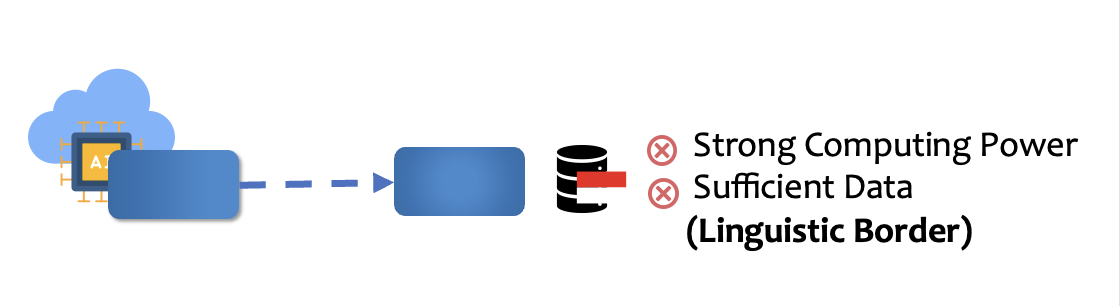
\includegraphics[width=\linewidth]{1.jpg}
            \caption{Monolingual Tuning.}
            \label{fig:a}
        \end{subfigure}
        \\
        \begin{subfigure}[b]{\linewidth}
            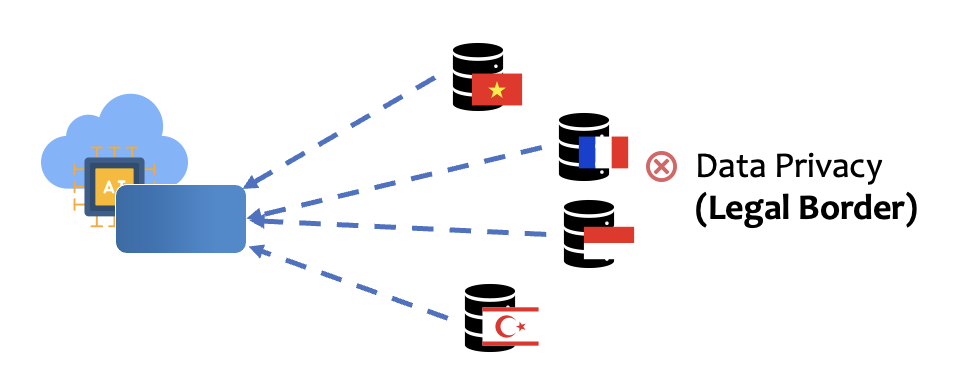
\includegraphics[width=\linewidth]{2.jpg}
            \caption{Centralized Tuning.}
            \label{fig:b}
        \end{subfigure}
    \end{minipage}
    %\hfill
    \begin{minipage}{0.49\linewidth}
        \begin{subfigure}[b]{1.1\linewidth}
            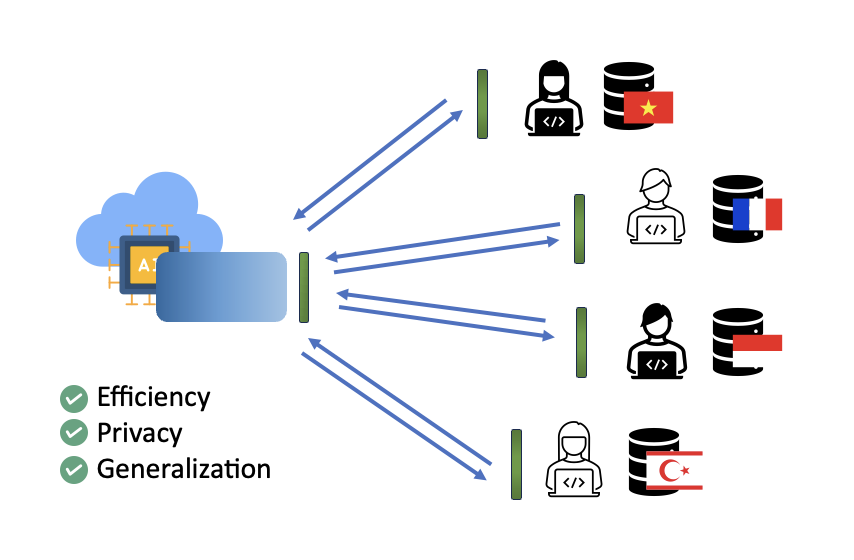
\includegraphics[width=\linewidth]{3.jpg}
            \caption{Federated Prompt Tuning.}
            \label{fig:c}
        \end{subfigure}
    \end{minipage}
    \caption{Comparison of three different fine-tuning paradigms for multilingual tasks. }
    \vspace{-0.5cm}%%压缩图片后间隔
    \label{fig:images}
    
\end{figure}
Federated learning (FL)~\citep{fedavg} allows edge devices to collaboratively learn a shared global model while keeping their private data locally on the device, thereby decoupling the ability to do machine learning from the need to store data in the cloud. There are nearly seven billion connected Internet of Things (IoT) devices and three billion smartphones around the world~\citep{lim2020federated}, potentially giving access to an astonishing amount of training data and decentralized computing power for meaningful research and applications. Most existing FL works primarily focus on supervised learning where the local private data is fully labeled. However, assuming that the full set of private data samples includes rich annotations is unrealistic for real-world applications~\citep{fedmatch, semifl, jin2020towards,yang2021federated}. 
Although for some applications of FL, such as keyboard predictions, labeling data requires virtually no additional effort, this is not generally the case. 

Acquiring large-scale labeled datasets on the user side can be extremely costly. For example, a large amount of unlabeled data is generated through interactions with smart devices in daily life, such as pictures or physiological indicators measured by wearables. These volumes of data make it impractical to mandate individual users to annotate the data manually. This task can be excessively time-intensive for users, or they may lack the requisite advanced knowledge or expertise for accurate annotation, particularly when the dataset pertains to a specialized domain such as medical data~\citep{yang2021federated}. The complicated process of annotation results in most user data remaining unlabeled, further leading to the conventional FL pipeline being unable to conduct supervised learning.
Recent studies of self-supervised learning in FL attempt to leverage unlabeled user data to learn robust representations~\citep{gao2022federated,rehman2022federated,rehman2023dawa}. However, the learned model still requires fine-tuning on labeled data for downstream supervised tasks.

%FL has a lot of unlabeled data 
% FL might experience a more pressing need to utilize the unlabeled dataset compared to centralised training. For example, for cross-device FL, where participants are individual smart devices, a large amount of unlabeled data is generated through interactions with these devices, such as photos or physiological indicators measured by wearables. These volumes of data make it unfeasible to require each user to manually label the data because labeling can be very time-consuming for the user or because users might not possess the sophisticated knowledge or expertise to annotate their private data correctly, especially for the situation when the dataset is highly professional in the specific domain like medical data ~\citep{yang2021federated}, or suppose we have a workout app that automatically evaluates and corrects users' posture. In this case, the end users may be unable to evaluate their posture to correctly label their private, but it is possible to have few limited data stored on the server that can be labeled by experts.

Compared to FL environments, centralized data annotation is more straightforward and precise in data centers. Even in low-resource contexts (e.g., medical data), the task of labeling limited data stored on the server by experts would not demand substantial effort. The integration of semi-supervised learning (SSL)~\citep{chapelle2009semi, yang2022survey,fixmatch,mixmatch} with FL can potentially leverage limited centralized labeled data to generate pseudo labels for supervised training on unlabeled clients. Existing work~\citep{jeong2020federated,zhang2021improving} attempted to perform SSL by using off-the-shelf methods only, such as FixMatch~\citep{fixmatch}, MixMatch~\citep{mixmatch} in FL environments. Although these methods provide certain model convergence guarantees during the FL stage, they cause heavy traffic for data communication due to their per-mini-batch communication protocol. Another recent work, SemiFL~\citep{semifl}, improves the training procedure by implicitly conducting entropy minimization. This is achieved by constructing hard (one-hot) labels from high-confidence predictions on unlabeled data, which are subsequently used as training targets in a standard cross-entropy loss. However, it is argued that using pseudo-labels based on model predictions might lead to a confirmation bias problem or overfitting to easy-to-learn data samples~\citep{nguyen2023boosting}. In addition, the existing methods typically establish a pre-defined threshold, generally set relatively high, to retain only samples with very high confidence.
This might lead to slow convergence issues, especially during the beginning of training when there are very limited samples satisfying the threshold.

In this paper, we propose an enhanced federated SSL method, dubbed \method ~- a newly designed label contrastive loss based on the cosine similarity metric to train on labeled anchor data on the server.
In this way, instead of retaining the high-confidence data through solely model prediction in the conventional SSL studies, \method \textit{for-the-first-time} generates the pseudo labels by comparing the similarities between the model representations of unlabeled data and label anchor data. This provides better quality pseudo-labels as shown in Fig.~\ref{fig:pip} (right), alleviates the confirmation bias, and reduces over-fitting easy-to-learn data issues. Our contributions are summarized as follows: 1) we propose a \textit{unique} pseudo-labeling method \method for SSL in FL, which leverages the similarities between feature embeddings of unlabeled data and label anchor data; 2) we design a novel label contrastive loss to further improve the quality of pseudo labels; 3) we perform extensive experiments on three different datasets having different sizes of labeled anchor data and show that the proposed methods achieve the state-of-the-art performance and faster convergence rate.


\begin{figure}[t!]
    \centering
    \begin{minipage}{0.55\linewidth}
        \centering
        \scalebox{0.75}{
        \begin{tabular}{l|ccccc|c}
        \toprule
        \bf Method & \bf en & \bf es & \bf fr & \bf de & \bf ru & \bf Avg \\
        \midrule
        Monolingual & 92.4&84.7&79.5&88.3&89.0& 86.8\\
        Centralized & 93.9 &86.7 &\bf 82.9 &\bf 89.5 &88.6 &88.3 \\
        FL (IID) & \bf 94.1& \bf 86.9&82.7& 89.4&\bf 88.8&\bf 88.4\\
        FL (Non-IID) &92.4&86.3&81.2&88.9&84.7&86.7\\
        \midrule
        PE\_Monolingual & 82.9& 59.7&47.3&71.4&60.0& 64.3\\
        PE\_Centralized & 89.1&76.2&67.4&78.8&75.9&77.5 \\
        PE\_FL (IID) \bf(Ours)&\bf 91.2&\bf 82.2&\bf 76.5&\bf 86.4&\bf 81.6&\bf83.6\\
        PE\_FL (Non-IID) \bf(Ours)&87.8&79.2&73.7&83.1&79.5&80.7\\
        \bottomrule
        \end{tabular}
        }
        \captionof{table}{Results for FL experiments on the NC task. Bold scores indicate the best in the column. }
        \label{tab:nc_main}
        \captionsetup{font=small,labelfont=bf}
    \end{minipage}%
    \hfill
    \begin{minipage}{0.43\linewidth}
        \centering
        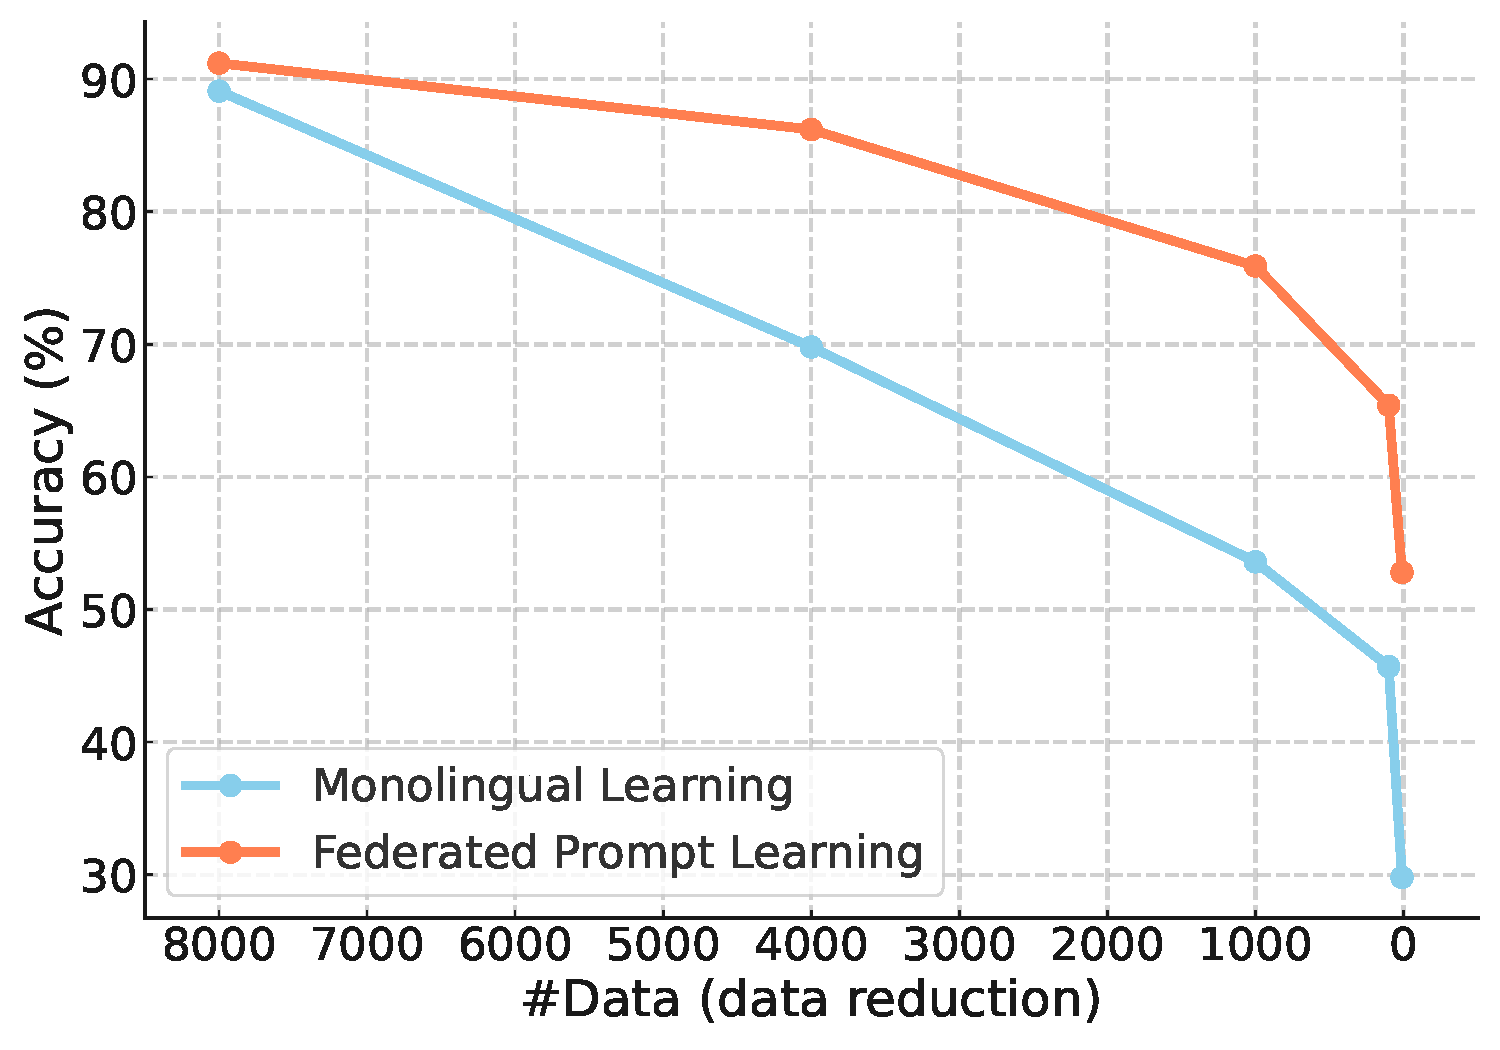
\includegraphics[width=\linewidth]{figures/data_efficiency.pdf}
        \caption{Performance comparison on NC with decreasing dataset size.}
        \label{fig:data_amount}
    \end{minipage}
    \vspace{-0.5cm}%%压缩图片后间隔
\end{figure}

\\
\begin{table}[t!]
\centering
\caption{Results for FL experiments on the XNLI task. Bold scores indicate the best in the column. The PE\_FL is evaluated under the Non-IID setting. }%All experiments are reported with 1 setup phase and 5 training rounds, and each experiment is repeated 10 times, and averages and standard deviations are reported.}
\captionsetup{font=small,labelfont=bf}
\label{tab:xnli_main}
\scalebox{0.7}{
%\resizebox{\textwidth}{!}{%0.8\textwidth
%\begin{tabular}{c|P{1.2cm}P{1.1cm}P{1.1cm}P{1.1cm}P{1.2cm}P{1.2cm}P{1.2cm}P{1.2cm}}
\begin{tabular}{l|ccccccccccccccc|c}
\toprule
\bf Method & \bf en & \bf fr & \bf es & \bf de & \bf el & \bf bg & \bf ru & \bf tr & \bf ar & \bf vi & \bf th & \bf zh & \bf hi & \bf sw & \bf ur & \bf Avg\\
\midrule
Monolingual & 39.1&35.1&36.6&35.7& 35.3&35.9&35.5&26.2&32.1&31.7&31.5&33.7&31.6&26.0&28.1& 32.94 \\
Centralized & 35.3&36.9&33.3&35.3&30.5&36.5&33.7&35.7&33.3&\bf 40.1&36.1&30.5&37.3&\bf 38.6&29.3&34.86 \\
% PE\_FL (IID)&91.2&82.2&76.5&86.4&81.6&83.58\\

PE\_FL \bf(Ours)&\bf 43.2&\bf 40.6&\bf 42.9&\bf 40.2&\bf 39.7&\bf 40.8&\bf 41.1&\bf 37.6&\bf 39.1& 39.9&\bf 39.4&\bf 39.8&\bf 38.2&37.1&\bf 37.8&\bf 39.83\\

\bottomrule
\end{tabular}
}
\vspace{-0.5cm}%%压缩图片后间隔
\end{table}




\begin{figure}[h]
    \centering
    \vspace{-0.3cm}%%压缩图片后间隔
    \begin{subfigure}{0.49\textwidth}
        \centering
        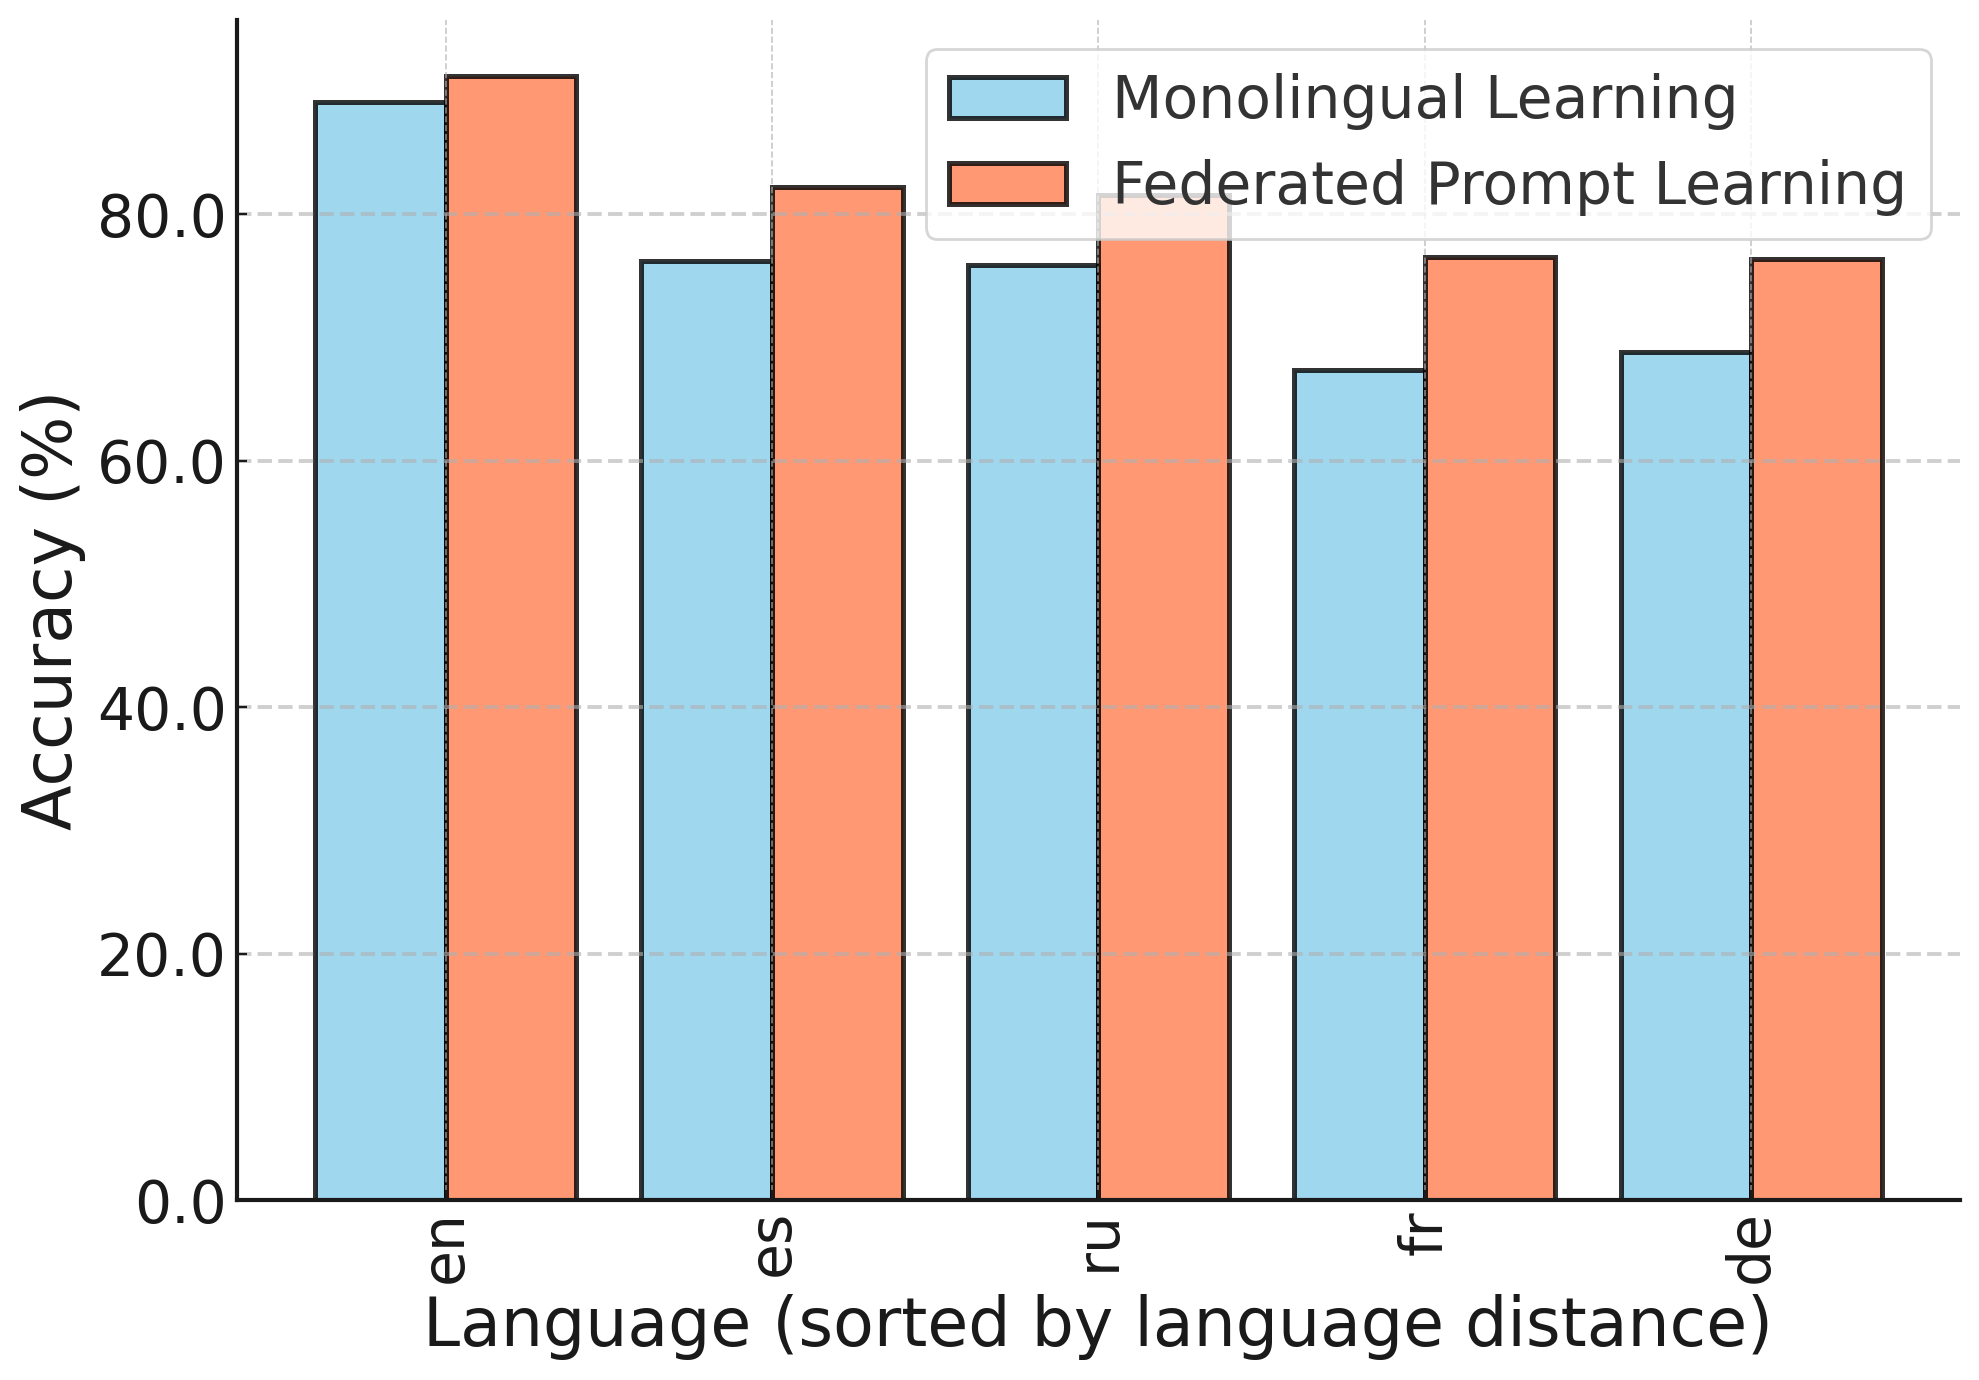
\includegraphics[width=0.8\linewidth]{figures/nc_lang.png}
        \vspace{-0.1cm}
        \caption{Finetuning accuracy across different lanugages on the NC task. }
    \end{subfigure}
    \hfill
    \begin{subfigure}{0.49\textwidth}
        \centering
        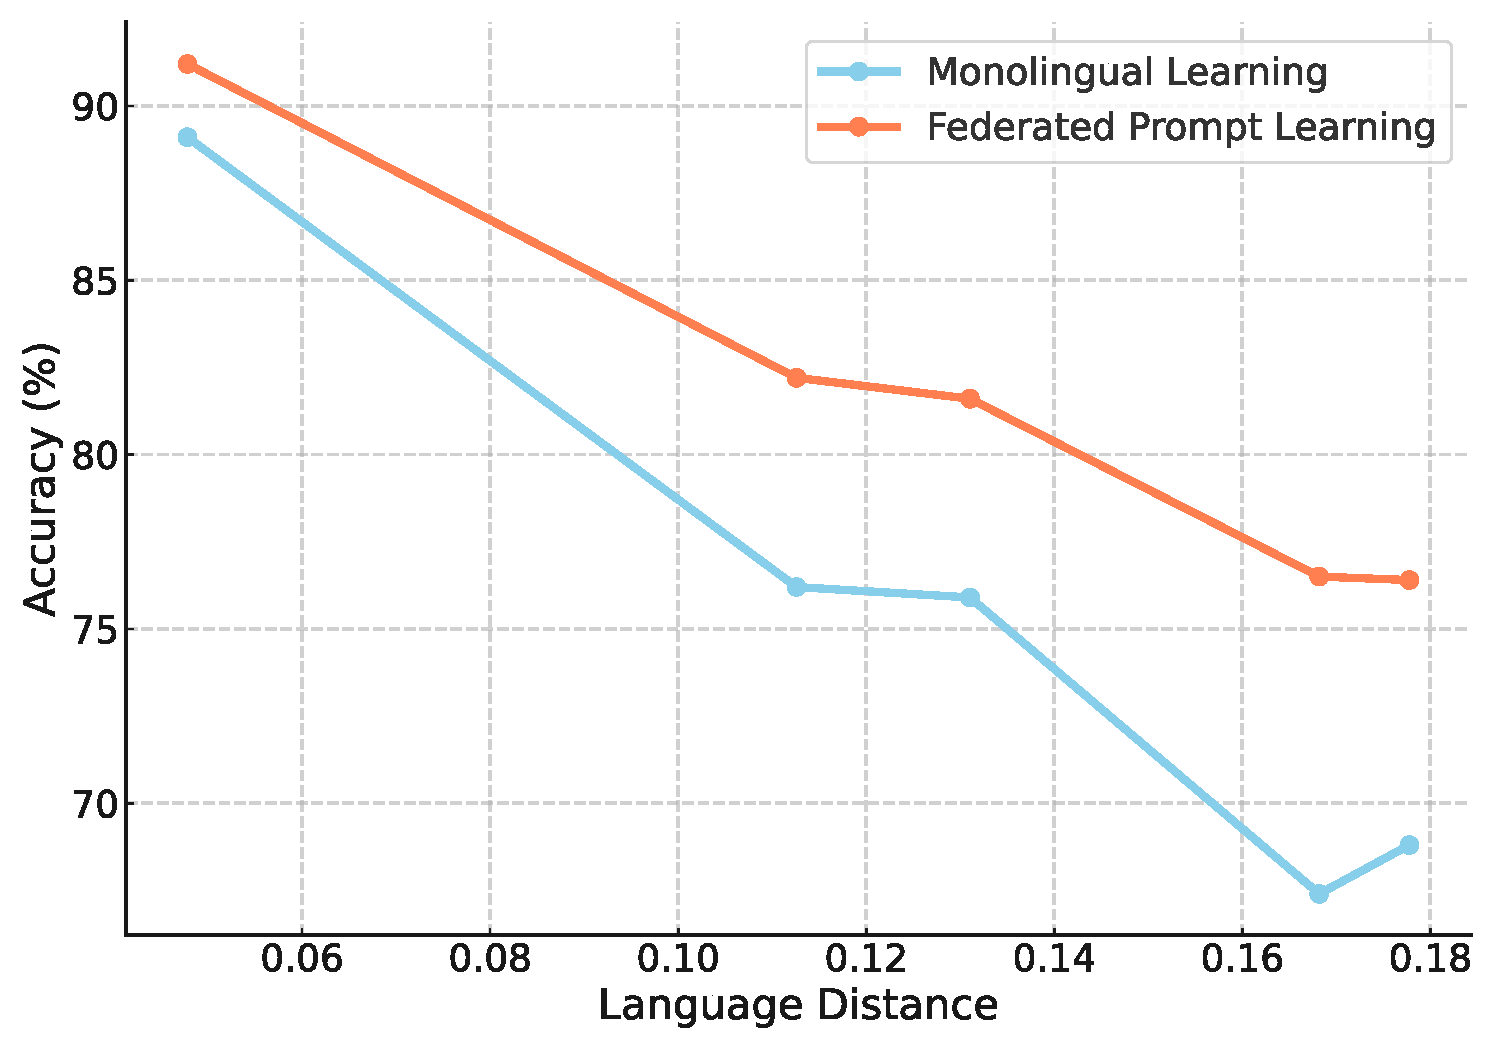
\includegraphics[width=0.8\linewidth]{figures/nc_distance.pdf}
        \vspace{-0.1cm}
        \caption{Finetuning accuracy across languages with varying similarity to the pre-trained language on the NC task. }
    \end{subfigure}
    \hfill
    \begin{subfigure}{0.49\textwidth}
        \centering
        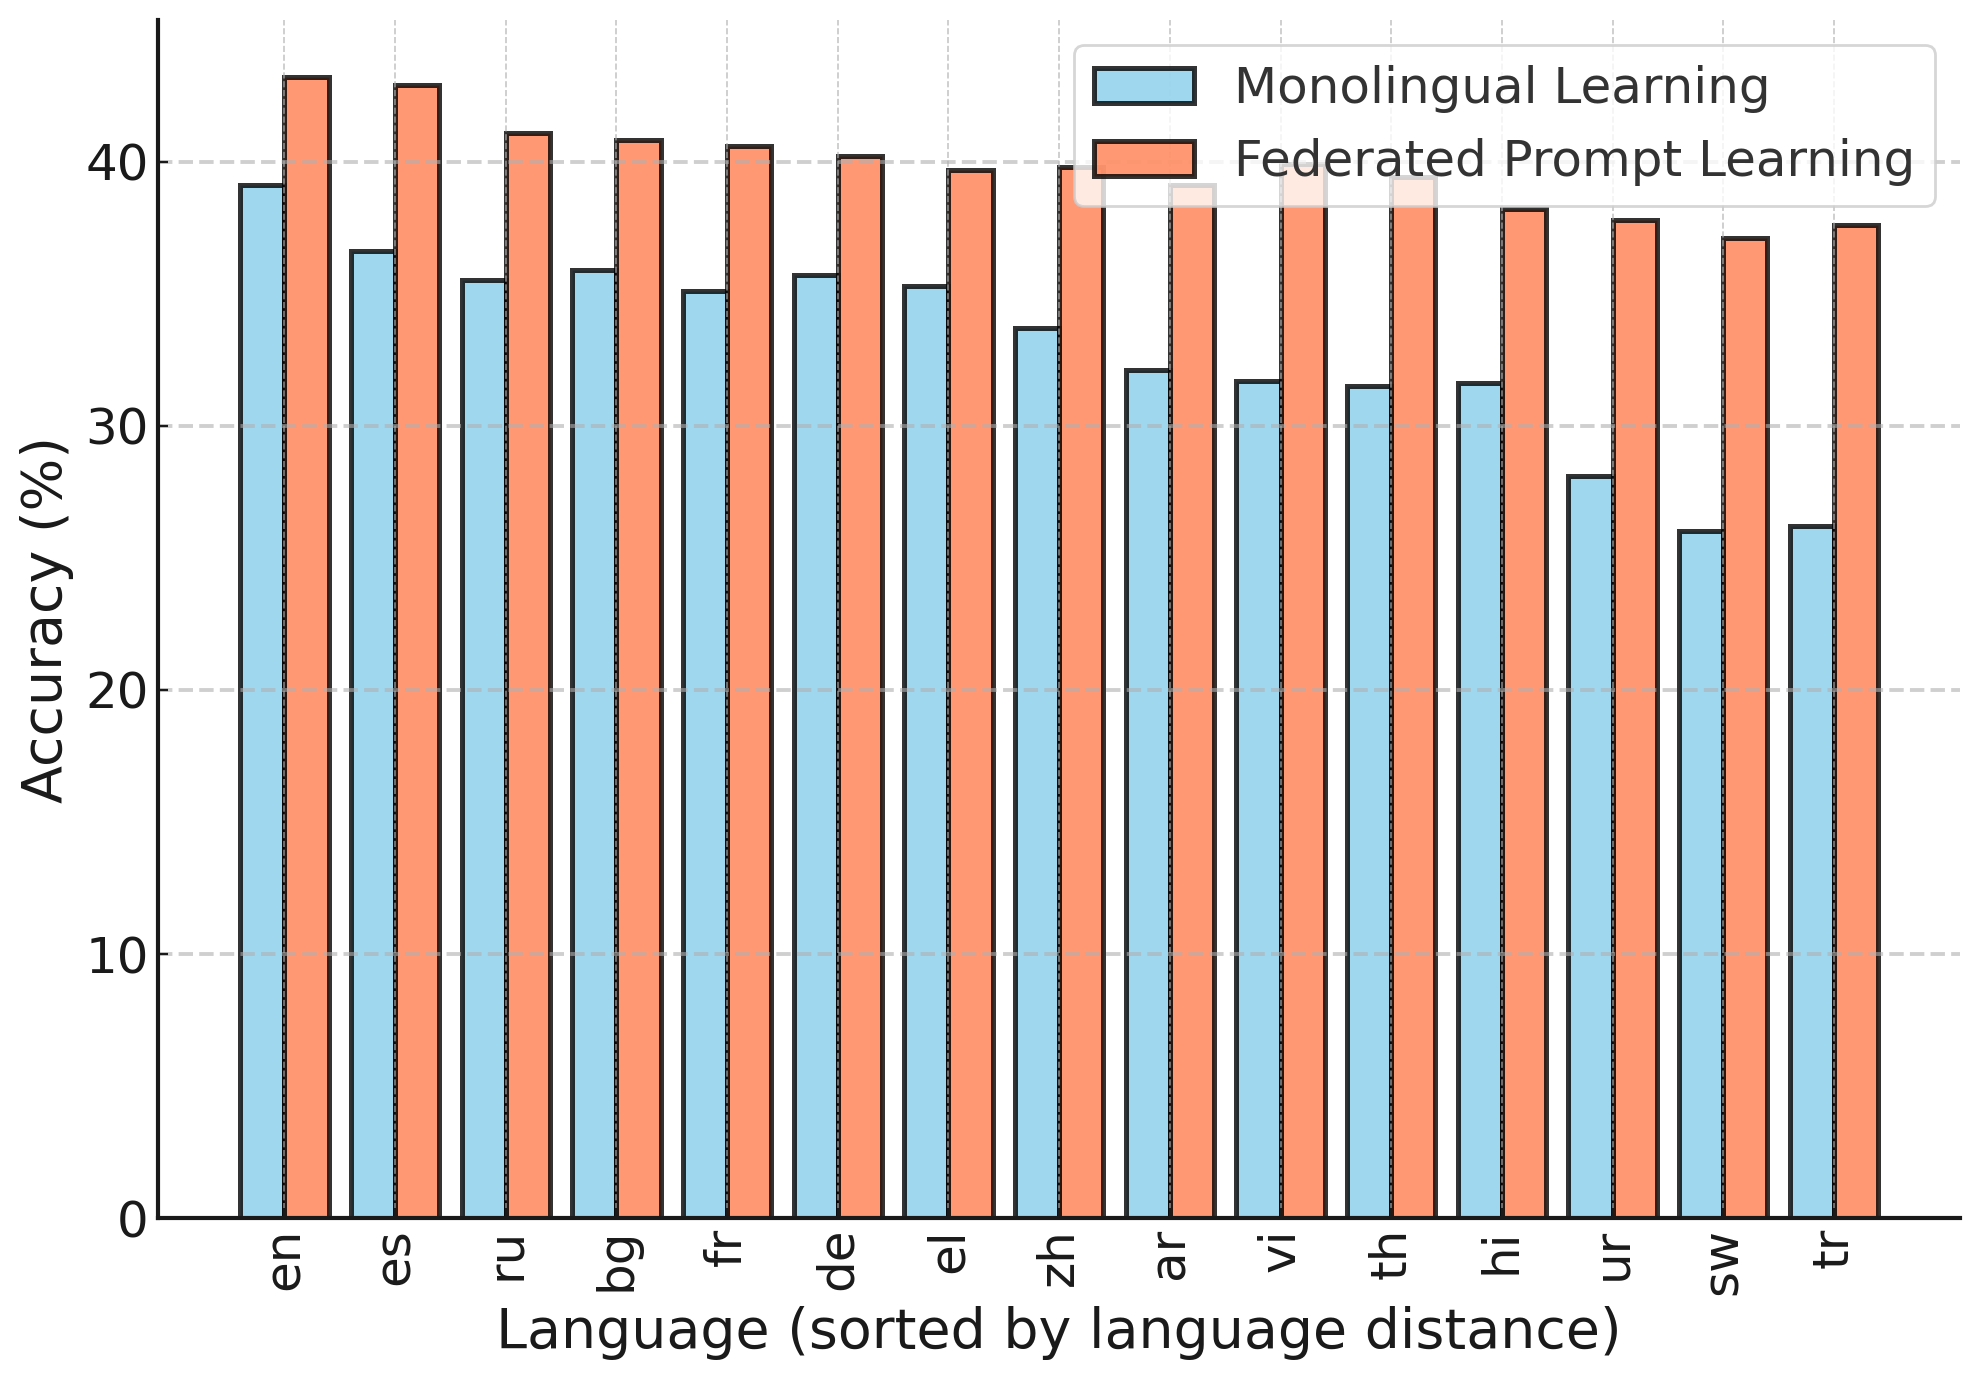
\includegraphics[width=0.8\linewidth]{figures/performance-distance-xnli.png}
        \vspace{-0.1cm}
        \caption{Finetuning accuracy across different lanugages on the XNLI task. }
    \end{subfigure}
    \hfill
    \begin{subfigure}{0.49\textwidth}
        \centering
        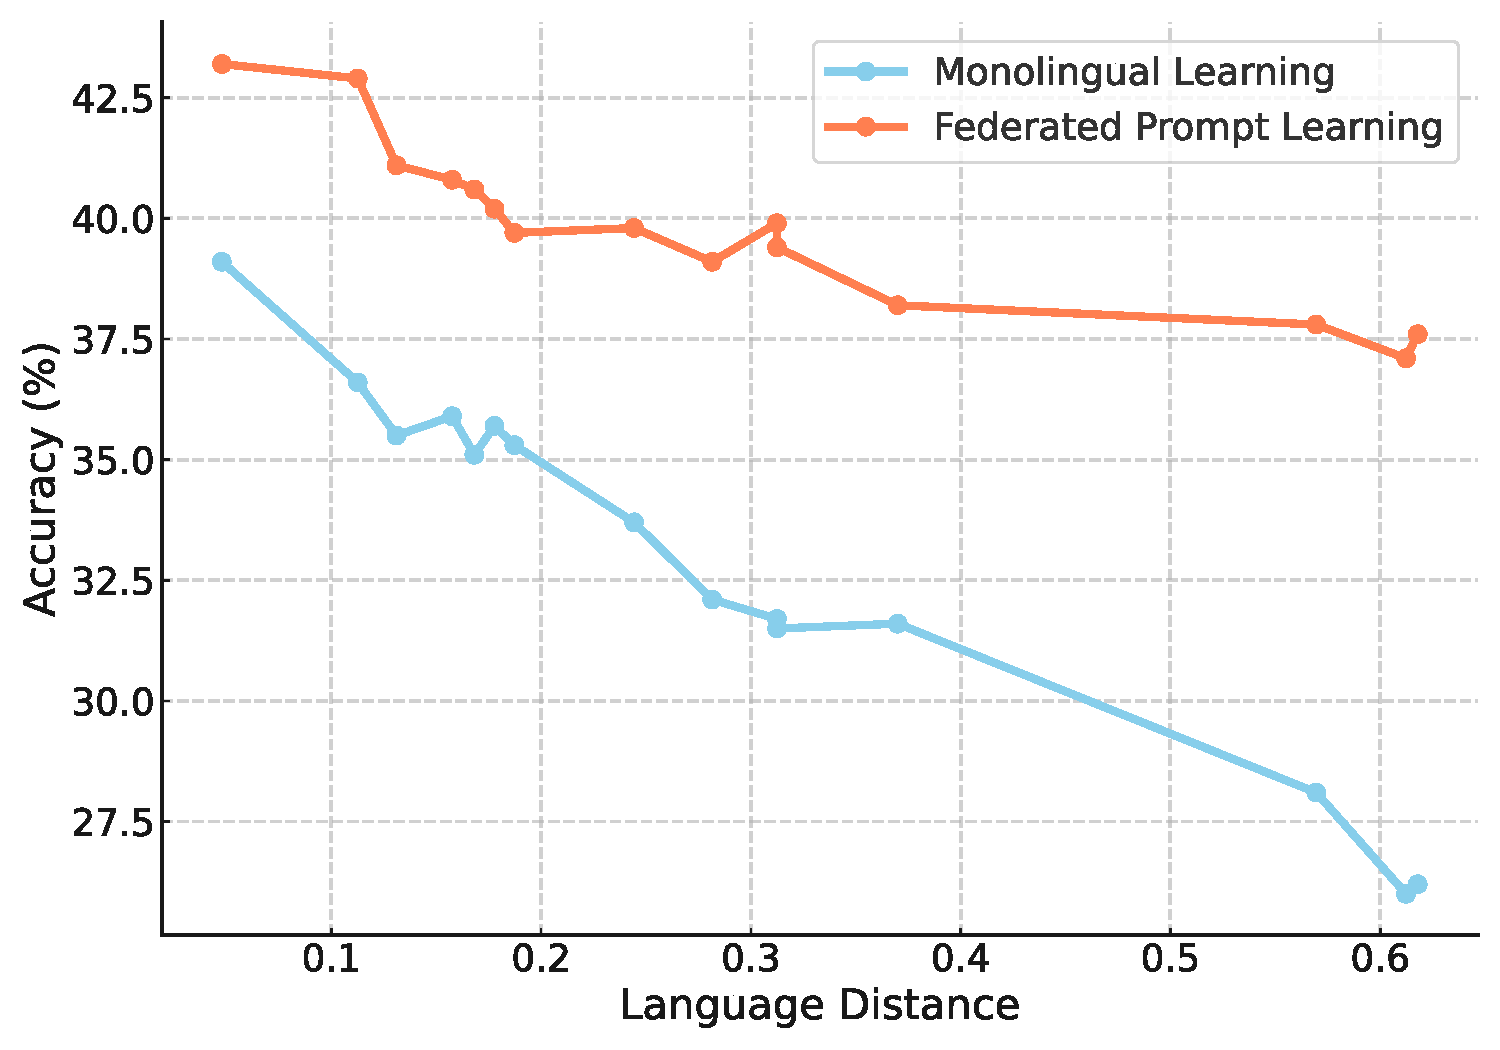
\includegraphics[width=0.8\linewidth]{figures/xnli_distance.pdf}
        \vspace{-0.1cm}
        \caption{Finetuning accuracy across languages with varying similarity to the pre-trained language on the XNLI task. }
    \end{subfigure}
    \caption{Comparative performance of traditional local finetuning and our Federated Prompt Tuning method across languages with varying similarity to the pre-trained language for XNLI and NC. }
    \vspace{-0.5cm}%%压缩图片后间隔
    \label{fig:combined}
\end{figure}

\begin{figure}[t]
\centering
    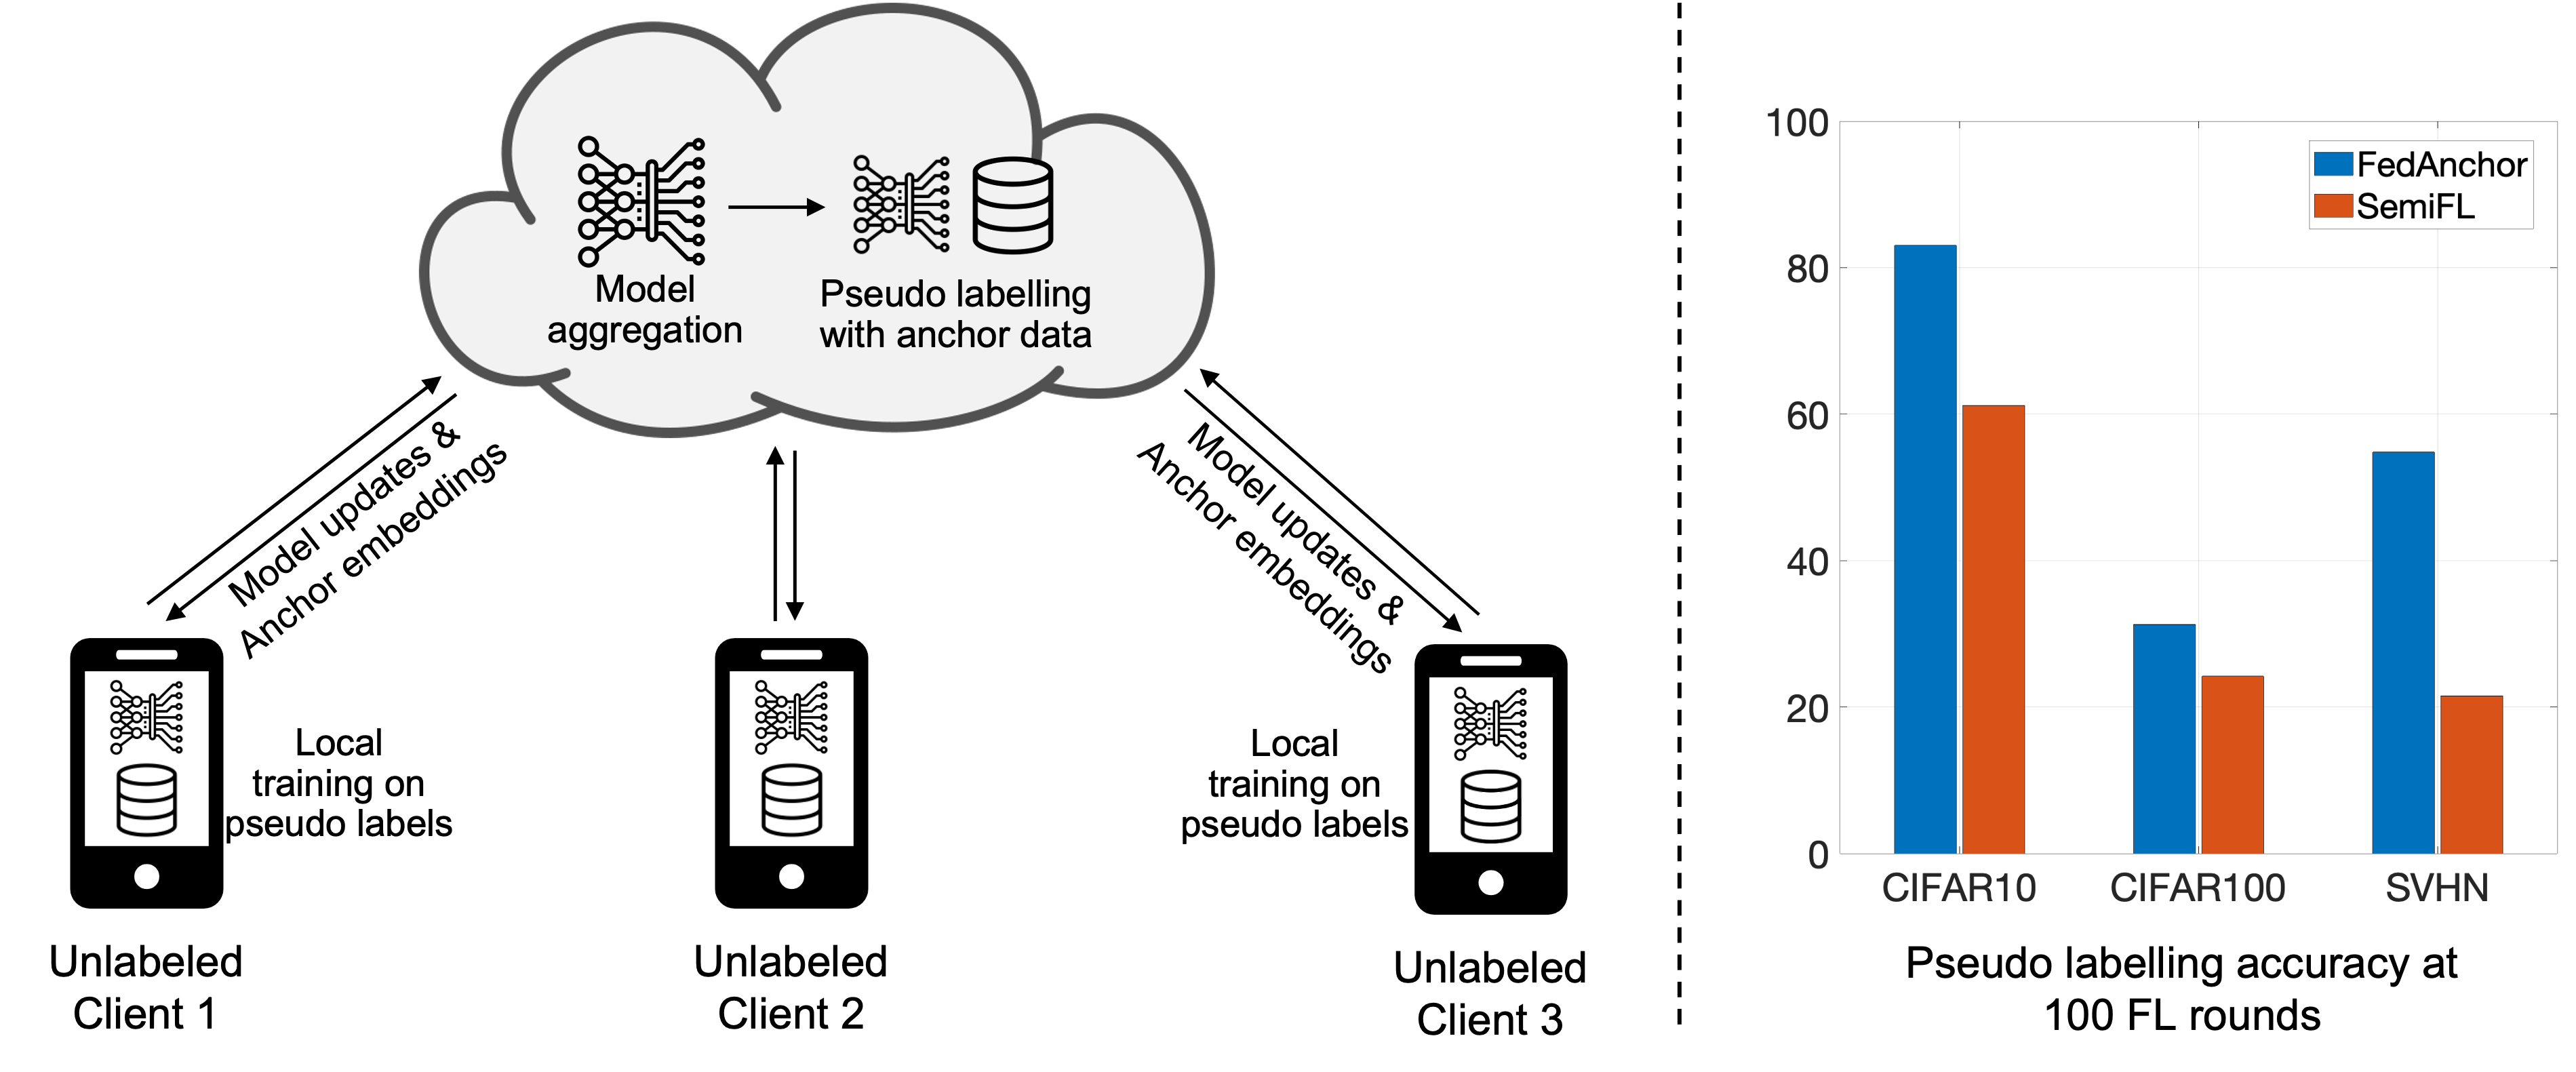
\includegraphics[width=\linewidth]{figures/pip.png}
\caption{\small (left) Pipeline of \method with pseudo labeling and anchor data on the server. Anchor embeddings are only transmitted to the clients during downstream communication. (right) Pseudo labeling accuracy with 5000/2500/1000 anchor data on CIFAR10/CIFAR100/SVHN datasets, respectively.}
\label{fig:pip}
\vspace{-5mm}
\end{figure}





% potentially more dataset stored on the server:
%Some medical datasets~\citep{yang2021federated} may require the most experienced experts to annotate their samples and also reduce the annotation burden under the distributed settings.




% this is why we need semi-supervised learning
% A powerful approach for training models on a large amount of data without requiring a large number of labels is semi-supervised learning (SSL)~\citep{chapelle2009semi, yang2022survey}. SSL mitigates the requirement for labeled data by providing various methods for leveraging the unlabeled data. Since unlabeled data can often be obtained with minimal human labor and limited human supervision, any performance boost conferred by SSL often comes with a low cost \citep{miyato2018virtual, sajjadi2016regularization, tarvainen2017mean}. A naive solution to these problems and challenges is to simply perform SSL using any off-the-shelf methods, such as FixMatch \citep{fixmatch}, MixMatch \citep{mixmatch}, UDA \citep{xie2020unsupervised}, etc.

% Standard communication efficient FL training \citep{fedavg}, each selected client can train multiple local epochs before sending the updated model parameters to the central server for aggregation, but taking the off-the-shelf SSL method and directly applying it to FL cannot achieve communication-efficient FL training. On the other hand, current methods mainly perform entropy minimization implicitly by constructing hard (1-hot) labels from high-confidence predictions on unlabeled data and using these as training targets in a standard cross-entropy loss. However, it is also argued that using pseudo-labels based on model predictions might lead to a confirmation bias problem or overfitting to easy-to-learn data samples \citep{nguyen2023boosting}. In addition, the current method [\textbf{REF}] normally sets a pre-defined threshold, which usually is quite high only to retain the very high-confidence samples. This might lead to slow convergence issues, especially during the beginning of training when there are very limited samples satisfying the threshold.

%constrastive loss \citep{simclr}


% There are generally two scenarios of FSSL \cite{fedmatch}. The first is called \textit{label-at-client}, where clients have both labeled and unlabeled data, and the second case is \textit{label-at-server}, where all labeled/anchor data are stored on the server, while all clients have only unlabeled data. \textit{label-at-server} is considered a more challenging case among these two. This work considers the opportunities of federated semi-supervised learning with the more challenging scenarios when the labeled dataset solely exists on the server. We propose \method and provide the following contributions:

% \begin{itemize}
%     \item We propose a unique double-head structure, with one \textit{Anchor head} attached with a newly designed label contrastive loss based on the cosine similarity to train on labeled anchor data on the server while keeping that originally \textit{Classification head} trained by both unlabeled client data and label anchor data. In this way, instead of retaining the high-confidence data through solely model prediction, we obtain the pseudo label by comparing the similarities between unlabeled data and label anchor data to provide better quality pseudo-labels, while alleviating the confirmation bias and over-fitting easy-to-learn data problems.
%     %\item innovative label contrastive loss designed for better quality pseudo labels
%     \item We perform extensive experiments on three different datasets with different sizes of labeled anchor data on the server and show that \xq{input significant results here. }    
% \end{itemize}



\subsection{Early Exit Project}
%%%

Self-supervised learning (SSL) has achieved state-of-the-art (SOTA) results in numerous tasks, which typically benefit from vast amounts of unlabelled training data.  With the advancement of the internet of things (IoT), a substantial amount of user data, with the nature of privacy-sensitive and unlabelled, is generated daily from edge devices. 

Federated learning (FL) can be harnessed to leverage this user data, enabling the learning of more robust representations. However, SSL models are typically large in size and notoriously resource-intensive to train, posing a challenge due to the diverse computational capabilities of client devices, some of which may not support the training of SSL models.

*How do we train an SSL model in heterogeneous FL settings with different hardware for each client? How can we transfer the knowledge from the client’s models to a single global model for a more robust representation learning?* These are important and fundamental questions for SSL in FL.

The proposal is to train SSL models with FL in a setting in which clients have different hardware. We don’t care about what happens after the training, and we want each client to contribute to improving the knowledge of the global model.

The pieces of **novelty** compared to ScaleFL and other works would be:

- We focus on **SSL models**, i.e. the final output of our procedure is a global full model that can be used for downstream tasks. Possibly, the trained early exit networks can be used as well. In ScaleFL, the authors use ResNet, MSDNet (multi-exit CNN architecture), and pre-trained BERT. ScaleFL is meant to work generally with models’ architectures allowing for 2-D model splitting and early exits.
- The objective is to optimise the model architecture configuration **dynamically** to match the edge device computational budgets. ScaleFL only clusters computational budgets once before training and assumes a specific linear dependency between budgets and the number of model parameters. So, the model architectures for each group are fixed.
- Considering an absolute and direct association between model configurations and clients’ budgets that does not need a full clients clustering before the beginning of the federated training. ScaleFL assumes that at least one client can operate on the full model, i.e. the group containing the most capable client is coupled with the full model. The other groups of clients are assigned to a corresponding level of complexity depending on their budgets at the beginning of the federated training. The levels of complexity are determined by a heuristic method.
- Improve the selection of the configurations compared to ScaleFL, which relies too much on structural dependencies of the weights in the network.
- Possibly improve the aggregation procedure compared to ScaleFL, which relies on the abovementioned structural dependencies and the self-distillation step.



\section{Federated Prompt Tuning}

Pretrained large language models (LLMs) have been driving the recent progress in natural language processing~\citep{brown2020language,chowdhery2022palm,anil2023palm,touvron2023llama,touvron2023llama2}. These large models, built on extensive corpora, offer valuable insights and impressive results across a range of applications. At the meantime, in order to provide universally accessible knowledge with LLMs, extending them to multiple languages has become a particularly relevant research target~\citep{XLM,XLM-R,artetxe-etal-2020-cross,pfeiffer-etal-2020-mad}. 

However, finetuning and deploying multilingual LLMs in practical downstream tasks are not as easy as its monolingual counterpart. First of all, sharing data across different regions can be difficult or even impossible. Regulations like the General Data Protection Regulation (GDPR) \cite{lim2020federated} limit cross-region data-sharing. Moreover, languages in various regions can be radically different, e.g. Sino-Tibetan and Indo-European, posing a Non-Independent and Identically Distributed (non-IID) challenge when learning a global multilingual model.
%
%
This situation accentuates privacy concerns, and highlights the need for effective privacy-preserving techniques when using multilingual LLMs. 
%
To this end, recent works attempt to address privacy-constrained fine-tuning for multilingual tasks and explore how different languages impact the FL training process ~\cite{Weller2022PretrainedMF}. 
%
However, they primarily target high-resources languages; research on low-resource languages remains largely unexplored.


Addressing low-resource languages is essential to promoting technological fairness and protecting the linguistic diversity. Unlike their high-resource counterparts, low-resources languages pose intriguing research challenges: 
%
i) \textbf{Limited computational resources.} Regions of low-resources languages are often economically developing areas, with little access to huge computational resources required to either train language models from scratch or fully fine-tune pre-trained large language models~\citep{mager2021findings,adebara-abdul-mageed-2022-towards}.
ii) \textbf{Limited data in the target language.} Due to a small speaking population or the spoken nature of the language, data is often scarce~\cite{adelani2021masakhaner,muhammad2022naijasenti,ebrahimi-etal-2022-americasnli}. As depicted in Figure ~\ref{fig:linguistic_coverage}, the pretraining data for LLMs is predominantly in English, with little coverage of low-resource languages. Under such circumstances, the performance of low-resources languages is often unsatisfactory during fine-tuning because of their under-representation.
iii) \textbf{Memorization risk.} Recent studies find that as pre-trained models scale up, their ability to memorize training data increases~\cite{tirumala2022memorization}. This implies that, when fine-tuning these models with limited data, the risk of overfitting and potential privacy issues arises.

To counteract the above challenges, we turn to federated learning (FL), where the model training is done across multiple decentralized devices or servers while the data is always kept localized~\cite{fedavg, fedprox, yang2019federated}. In a multilingual setting, FL becomes particularly natural, as data from diverse linguistic backgrounds can be sourced without compromising user privacy, and due to the geographical spread and inherent linguistic diversity of devices, data on each node is likely to exhibit non-IID distribution.

In this paper, in order to mitigate the physical border and the linguistic border of multilinguality, we propose a new paradigm grounded in FL, Multilingual Federated Prompt Tuning, focusing on parameter-efficient fine-tuning for multilingual tasks across various regions or devices. Specifically, our global encoder can discern language patterns and cluster languages via federated prompt averaging, which allows each client to benefit from others' data without direct access. This strategy requires minimal computational resources and significantly improves performance, particularly for low-resource languages. We demonstrate the effectiveness of our method on standard NLP tasks including New Classification and XNLI. The performance of our paradigm achieves 6.9\% accuracy improvement while protecting the privacy of mulitlingual source data. Compared with other Federated Learning approches, our paradigm reduces computational cost and communication cost by more than 99\%. Our approach paves the way for fine-tuning multilingual large language models on resource-constraint devices in a privacy-preserving way, and holds the potential to promote social equality, privacy, and linguistic diversity in the research community.


\begin{figure}
    \centering
    \vspace{-1cm}%%减小图片上间隔
    \begin{minipage}{0.49\linewidth}
        \begin{subfigure}[b]{\linewidth}
            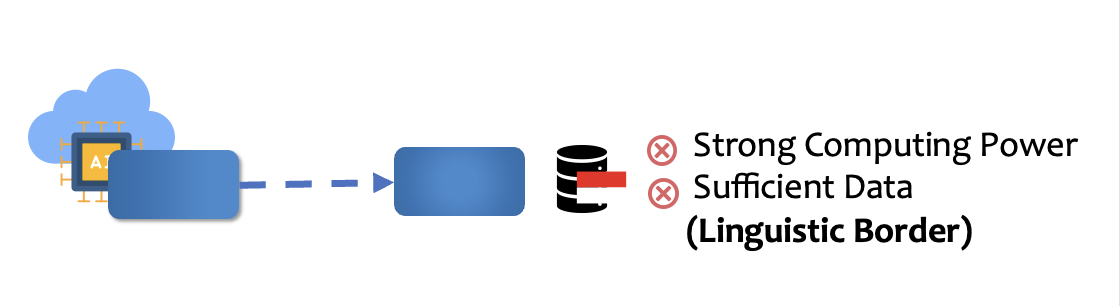
\includegraphics[width=\linewidth]{1.jpg}
            \caption{Monolingual Tuning.}
            \label{fig:a}
        \end{subfigure}
        \\
        \begin{subfigure}[b]{\linewidth}
            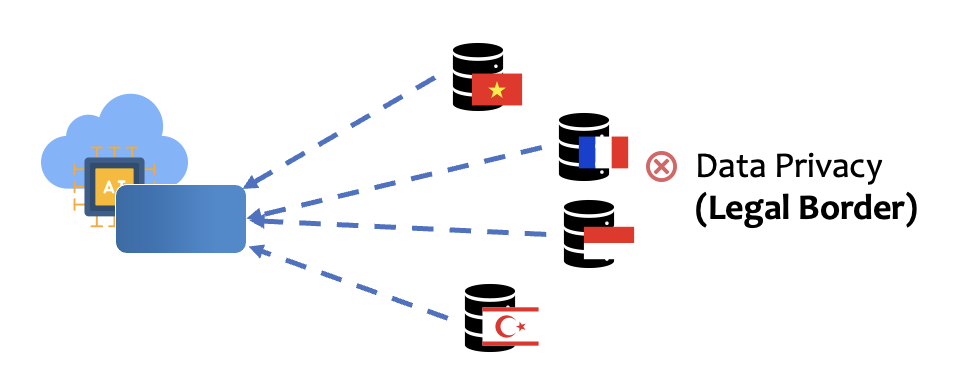
\includegraphics[width=\linewidth]{2.jpg}
            \caption{Centralized Tuning.}
            \label{fig:b}
        \end{subfigure}
    \end{minipage}
    %\hfill
    \begin{minipage}{0.49\linewidth}
        \begin{subfigure}[b]{1.1\linewidth}
            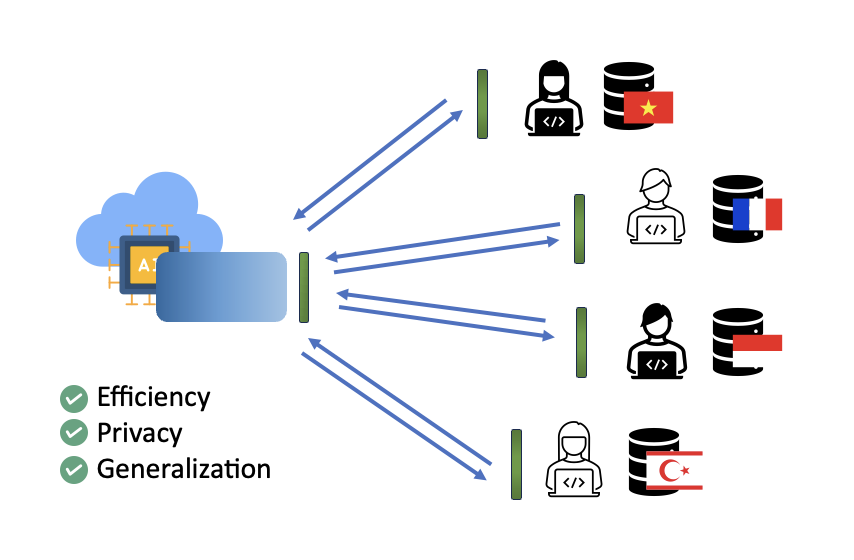
\includegraphics[width=\linewidth]{3.jpg}
            \caption{Federated Prompt Tuning.}
            \label{fig:c}
        \end{subfigure}
    \end{minipage}
    \caption{Comparison of three different fine-tuning paradigms for multilingual tasks. }
    \vspace{-0.5cm}%%压缩图片后间隔
    \label{fig:images}
    
\end{figure}


\chapter{Proposed Research} \label{Proposal}

\section{Data: Data Alignment for Federated Learning}

%\section{Domain Adaptation in Federated Learning}

\subsection{Data-Augmented FL}

One of the earlier known works to use dataset augmentation to relieve heterogeneity is FedShare [19], in which the server transmits real examples from a public dataset to clients. 

While only small number of examples are needed to significantly boost model performance, it is unrealistic to assume the server has examples for every or any label. In lieu of real examples, sample mixing is a popular augmentation strategy. Mixup [18] forms convex combinations of k examples (k-way mixup) and their labels, with weights drawn from common random distributions. Mixup and its privacy-improved variant InstaHide [5] produces pseudo-synthetic training data beneficial to improving model-robustness against adversarial examples.

FedMix [17] was one of the earlier known works to use mixup to balance label-skew. To homogenize data distributions, k-way mixups of all client data and labels are constructed and sent up to the server, where it is then unioned and sent back down to clients for training. This approach can prove expensive over large client clusters, especially if the total data size across all clients is massive, and for smaller, C = 1 label-skewed clients, their mixups are easily decodable by other clients with rich, balanced data [3] due to information gleaned from the ”pseudo”-label – which will contain one entry. XORMixFL [15] also distributes mixed-client data via mixup and is intended for one-shot server-side training, as opposed to directly improving local training.

Currently, the training of large-scale models heavily relies on public domain data. Recent studies indicate that the availability of such public data is nearing exhaustion. To further enhance the performance of large models, there is an urgent need to incorporate high-quality, domain-specific private data. However, due to their unique security and privacy attributes, private datasets become "accessible but invisible" resources. This poses significant challenges in quality control during model training. To address this, our research proposes a federated learning approach centered on data quality. By ensuring data privacy, we purposefully select multi-party private data that aligns with the "3H" principle (Helpful, Honest, Harmless) for language model training. The goal is not only to improve model performance but also to ensure alignment with human values.

Technical Roadmap:

Starting from quantifying the contribution of samples to model performance, we design an impact function to effectively identify and eliminate samples that compromise the model's performance and safety, enhancing both the overall model performance and human-machine alignment.

For the federated model training scenario, we propose a client-based distributed filtering and aggregation algorithm. This ensures data privacy while filtering data according to the "3D" principle.

We introduce a rapid retraining technique based on meta-learning and machine forgetting. Without compromising the model's performance, this enhances the safety and human-machine alignment in multi-party collaborations.


\subsection{Dataset Shift} 

% Domain Adaptation
% https://www.youtube.com/watch?v=iLT08YG2Mt0

\section{Model: Incentive Machinism}

\section{Memory: Efficient Federated Learning}

% Personalized Federated Learning Memory Budget

% Dynamic Neural Network

% The name EfficientNet suggests that the architecture is very efficient, but in what sense? There are many types of ‘efficiency’, but let’s consider two of them: parameter efficiency and computational efficiency.

Parameter efficiency tries to optimize the ratio between the model performance (e.g. accuracy) and the amount of parameters used. Models which are efficient in terms of the amount of parameters tend to require less data to train and generalize better.

Computational efficiency tries to optimize the ratio between model performance and the amount of computational time that needs to be spent. Depending on what is most crucial, computational efficiency could be calculated based on the time required to train the model, or the time required to do inference.


% Memory

Large language models (LLMs) have become a cornerstone of natural language processing (Brown et al., 2020; Touvron et al., 2023a; OpenAI, 2023; Anil et al., 2023), and fine-tuning pre-trained LLMs has been shown very effective to improve their performance in various downstream tasks (Liu et al., 2019; Wei et al., 2021) and to enable them to align with human intents (Ouyang et al., 2022; Bai et al., 2022). However, fine-tuning LLMs with full parameter is prohibitively expensive, for example, fine-tuning a LLaMA-65B (Touvron et al., 2023a) model with AdamW (Loshchilov & Hutter, 2017) requires more than 1TB of GPU memory to store model parameter, gradient, and optimizer states (Rajbhandari et al., 2020).

To reduce the memory of full-parameter fine-tuning, parameter-efficient fine-tuning (PEFT) methods are proposed to update only a small fraction of parameters, such as adapter weights (Houlsby et al., 2019; Hu et al., 2022) and prompt weights (Li & Liang, 2021; Lester et al., 2021). Among these methods, LoRA (Hu et al., 2022) has shown to achieve comparable performance than full-parameter fine-tuning, and it has been widely used in many applications (Dettmers et al., 2023).
Specifically, LoRA adds a parallel low-rank adapter besides the weight of a linear layer, as shown in Figure 1(b), where W is the pre-trained weight, A and B are low-rank weights. Because LoRA freezes W and only updates smaller matrices A and B, its memory overhead for trainable parameter and corresponding gradient and optimizer states can be largely reduced, compared to full-parameter fine-tuning as shown in Figure 1(a), which can be regarded as updating W and freezing A and B. Furthermore, LoRA introduces no additional inference latency by merging the value of AB into W. However, LoRA still has limitations as it requires expensive activation memory consumption in LoRA layers. This is because the large input activation of X needs to be stored during the feed- forward pass, and used to construct the gradient of A during the back-propagation pass. It means LoRA cannot reduce the activation memory cost compared to full-parameter fine-tuning. For ex- ample, fine-tuning a LLaMA-65B with input sequence length of 2048 and batch size of 4 requires more than 50GB of activation memory (in 16-bit format) in all LoRA layers. To address it, existing methods select a part of linear layers for LoRA fine-tuning (Hu et al., 2022) or use activation recom- putation (Chen et al., 2016), which however could affect fine-tuning performance or efficiency.


% \section{Communication}

% 未来 LLM 算法研究也必然朝着 Infra 的方向去探索: 稀疏化(Sparse Attention、 Sparse GEMM / MoE) 将会是明年的(学术界/工业界)主战场。 即使是 Dense 的大模型(LLaMa2), 也在探索诸如 GQA (Grouped Query Attention) 等算法结构上的调优,这些算法优化并不是为了提升模型的效果,而是希望成倍的节省 Inference 时的 KVCache 显存,从而使 LLM 可以有更高的吞吐。

% 这个模型结构是否更容易分布式并行? 新的结构在各种并行时所需的通信量是不是更低?
% 新的模型算法是否拥有: 更少的计算量、 更少的显存需求、 更容易推理?
% 新的模型在做超长上下文(100K 以上的 Sequence Length) 时,如何训练 和 如何推理?

% 而在本来更加重要的方向,诸如 MoE ,只有少之又少的几篇经典 paper (Switch-T 、 GLaM)可以粗略的了解了解算法。 而 Infra 更是落后 OpenAI 数个版本(我不认为诸如 MegaBlocks、 Tutel、DeepSpeed-MoE 有能 Scale 到数千卡以上规模的能力),连一个最佳实践都没有。 这些具有巨大价值的 Know-how 被锁在了极少公司的核心团队内部。 OpenAI 从不热衷于写论文(可以改名为 CloseAI), Google 也开始 follow 了。


%DeepSpeed-MoE 通篇不提 PP,用 ZeRO 和 ZeRO Offload 去 scale,搞错了方向。

% Tutel / Megatron 对于 EP 的 Group 应该在哪个维度设计的不合理, EP Size 绑定 DP + TP , 受限于 Expert Num, 没法 Scale 到 500 卡以上。

% MegaBlocks 是一个单机 8 卡的工作。

% 核心问题是 EP Group 应该怎么设计, EP 如何跟 DP、TP、PP 结合, 目前已知的开源方案都没有很好的解决这些问题。

\chapter{Timeplan} \label{Timeplan}

\section{Year 2}
\paragraph{Michaelmas Term} 

• Continue work on quantization by addressing immediate follow-ups from Degree- Quant work.

• Implement fast quantized GNN kernels for CPU and potentially other platforms (e.g. mobile or GPU).

• Extensive literature review on activation compression and sparsity. 
\paragraph{Lent Term} 

• Write up conclusions on follow ups to Degree-Quant; if possible, written up early for a conference submission.

• Clean up quantization code and open source as a library.

• Begin work on activation compression. This work may be applicable to other types of architectures, so should evaluate on both GNNs and CNNs or Transformers.
\paragraph{Easter Term}

• Write up conclusions from activation compression project.

• Update library and open source.

• Explore follow-ups to activation compression project or assess other types of graph optimisations.

\paragraph{Summer Term}

• Buffer time for over-runs from previous projects, or if compelling follow-ups are worth exploring.

• Begin literature review on architecture design.

• Implement ideas to improve GNN architectural efficiency and write up for submission if promising results.

\section{Year 3}

\paragraph{Michaelmas Term}
• Finalise literature review for thesis.

• Continue work on GNN architectural efficiency if needed. Otherwise, assess follow-ups for any of previous work completed or choose an extension project.

• Keep library up to date.

\paragraph{Lent Term}

• Write up work from previous term.

• Begin thesis write-up.

• Write up summary of all projects and experiments completed.

• Continue work on outstanding projects.

\paragraph{Easter Term}
• Finalise projects. 

• Full thesis outline. 

• Continue write-up.

% Easter term would be devoted to finishing any work leftover from Michaelmas or Lent. The rest of the time will be devoted to constructing a complete thesis outline and continuing the write-up started during the Lent term. The summer term would be dedicated to finishing the thesis.

\paragraph{Summer Term}

% Thesis write-up, finish up outstanding experiments.
% Finish write-up, thesis submission, viva, corrections.
• Thesis write-up.


%%%%%%%%%%%%%%%%%%%%%%%%%%%%%%%%%%%%%%%%%%%%%%%%%%%%%%%%%%%%%%%%%%%%%%%%%%%%%%%%
%% References:
%%
% If you include some work not referenced in the main text (e.g. using \nocite{}), consider changing "References" to "Bibliography".
%

% \renewcommand to change default "Bibliography" to "References"
\renewcommand{\bibname}{References}
\cleardoublepage
\phantomsection
\addcontentsline{toc}{chapter}{References}
\bibliographystyle{plainnat}
\bibliography{thesis}



%%%%%%%%%%%%%%%%%%%%%%%%%%%%%%%%%%%%%%%%%%%%%%%%%%%%%%%%%%%%%%%%%%%%%%%%%%%%%%%%
%% Appendix:
%%

\appendix

\chapter{Extra Information}
Some more text ...



%%%%%%%%%%%%%%%%%%%%%%%%%%%%%%%%%%%%%%%%%%%%%%%%%%%%%%%%%%%%%%%%%%%%%%%%%%%%%%%%
%% Index:
%%
\printthesisindex

\end{document}
